% The % is a comment.  This file is an Example LaTeX document for GP111
\documentclass[11pt]{article}
\usepackage{times}                               % LaTeX 2e 
\usepackage{graphicx}
\usepackage{epstopdf}
%\usepackage{subfigure}
\usepackage[colorlinks=true]{hyperref}
%\usepackage[doublespacing]{setspace}

%%%%%%%%%%%%%%%%%%%%%%%%%%%%%%%%%%%%%%%%%%%%
% Generic Shared across papers Keywords

\newcommand{\fixme}[1]{{\Large FIXME:} {\bf #1}}
\newcommand{\note}[1]{{\bf Note:} \{\uline{#1}\}\\}

% create some additional spacing between paragraphs.
\setlength{\parskip}{7pt}
% Default margins are too wide all the way around.  I reset them here.
\setlength{\topmargin}{-.5in}
\setlength{\textheight}{9in}
\setlength{\oddsidemargin}{.125in}
\setlength{\textwidth}{6.25in}

\begin{document}

\title{OpenRAM Manual}
\author{Matthew R. Guthaus - mrg@ucsc.edu\\
  and many others
}
%\renewcommand{\today}{October 14, 2010}
\maketitle
\newpage
\section{License}

\begin{verbatim}
  Copyright 2018 Regents of the University of California and The Board
  of Regents for the Oklahoma Agricultural and Mechanical College
  (acting for and on behalf of Oklahoma State University)
  
  Redistribution and use in source and binary forms, with or without
  modification, are permitted provided that the following conditions are
  met:
  
  1. Redistributions of source code must retain the above copyright
  notice, this list of conditions and the following disclaimer.
  
  2. Redistributions in binary form must reproduce the above copyright
  notice, this list of conditions and the following disclaimer in the
  documentation and/or other materials provided with the distribution.
  
  3. Neither the name of the copyright holder nor the names of its
  contributors may be used to endorse or promote products derived from
  this software without specific prior written permission.
  
  THIS SOFTWARE IS PROVIDED BY THE COPYRIGHT HOLDERS AND CONTRIBUTORS
  "AS IS" AND ANY EXPRESS OR IMPLIED WARRANTIES, INCLUDING, BUT NOT
  LIMITED TO, THE IMPLIED WARRANTIES OF MERCHANTABILITY AND FITNESS FOR
  A PARTICULAR PURPOSE ARE DISCLAIMED. IN NO EVENT SHALL THE COPYRIGHT
  HOLDER OR CONTRIBUTORS BE LIABLE FOR ANY DIRECT, INDIRECT, INCIDENTAL,
  SPECIAL, EXEMPLARY, OR CONSEQUENTIAL DAMAGES (INCLUDING, BUT NOT
  LIMITED TO, PROCUREMENT OF SUBSTITUTE GOODS OR SERVICES; LOSS OF USE,
  DATA, OR PROFITS; OR BUSINESS INTERRUPTION) HOWEVER CAUSED AND ON ANY
  THEORY OF LIABILITY, WHETHER IN CONTRACT, STRICT LIABILITY, OR TORT
  (INCLUDING NEGLIGENCE OR OTHERWISE) ARISING IN ANY WAY OUT OF THE USE
  OF THIS SOFTWARE, EVEN IF ADVISED OF THE POSSIBILITY OF SUCH DAMAGE.
\end{verbatim}


\newpage
\setcounter{tocdepth}{2}
\tableofcontents

\newpage

% Each chapter description
%%%%%%%%%%%%%%%%%%%%%%%%%%%%%%%%%%%%%%%%%%%%%%%%%%%%%%%%%%%%%%%%%%%%%%%%%%%
\section{Introduction}
\label{sec:intro}

The OpenRAM project aims to provide a free, open-source memory
compiler development framework for Random-Access Memories (RAMs).
Most academic Integrated Circuit (IC) design methodologies are
inhibited by the availability of memories.  Many standard-cell process
design kits (PDKs) are available from foundries and vendors, but these
PDKs do not come with memory arrays or compilers. Some PDKs have
options to request ``black box'' memory models, but these are not
modifiable, have limited available configurations, and do not have
full details available to academics. These restrictions make
comparison and experimentation with real memory systems impossible.
OpenRAM, however, is user-modifiable and portable through
technology libraries to enable experimentation with real-world
memories at a variety of performance points and costs.

The specific features of OpenRAM are:
\begin{itemize}

\item \textbf{Memory Array Generation} 

  Currently, OpenRAM includes features such as automatic word-line
  driver sizing, efficient decoder sizing, multiple-word column
  support, and self-timing with replica bitlines.

\item \textbf{Portability and Extensibility} 

  OpenRAM is a Python program. Python enables portability to numerous
  platforms and enables the program to be extended by anyone. In
  general, it works on Linux, MacOS, and Windows platforms.

  User-readable technology files enable migration to a variety of
  process technologies. Currently, an implementation in a
  non-fabricale 45nm technology (FreePDK45) is provided and the MOSIS
  Scalable CMOS (SCN3ME\_SUBM.30) is provided. The compiler has also
  been extended to several technologies. We hope to work with vendors
  to distribute the technology information of others commercial
  technologies soon.

  OpenRAM makes calls to both open-source or commercial circuit
  simulators and DRC/LVS tools in an abstracted way for circuit
  simulation and verification. This enables adaptation to other design
  methodologies. It supports a completely open-source
  platform for older SCMOS technologies.

\item \textbf{Timing and Power Characterization}

  OpenRAM provides a basic framework for analysis of timing and power.
  This includes both analytical estimates, un-annotated spice
  simulations, or back-annotated simulations.  The timing and power
  views are provided in the Liberty open format for use with the most
  common logic synthesis and timing analysis tools.

\item \textbf{Commercial Tool Independence and Interoperability}

  To keep OpenRAM portable and maximize its usefulness, it it
  independent from any specific commercial tool suite or
  language. OpenRAM interfaces to both open-source (e.g., NGSpice) and
  commercial circuit simulators through the standard Spice3 circuit
  format. The physical layout is directly generated in the GDSII
  layout stream format which can be imported into any academic or
  commercial layout tools. We provide a Library Exchange Format (LEF)
  file for interfacing with commercial Placement and Routing tools.
  We provide a Verilog behavioral model for simulation.

\item \textbf{Silicon Verification} 
  TBD

\end{itemize}

\subsection{Requirements}

Development is done on Ubuntu or MacOS systems with Python 2.7. It
requires a few common Python libraries such as numpy, scipy (soon, for
optimization) along with standard Python libraries (os, sys, etc.).


\subsubsection{Timing Verification Tools}

For peformance reasons, OpenRAM uses analytical delay models by
default. If you wish to enable simulation-based timing
characterization, you must enable this on the command line with the
``-c'' command line argument.

% Not complete yet
%If you wish to perform back-annotated characterization, you must
%further enable this with the ``-b'' command line argument.

OpenRAM can use the following circuit simulators and possibly others
if they support the Spice3 file format:
\begin{itemize}
  \item HSpice I-2013.12-1 or later
  \item ngspice 26 \url{http://ngspice.sourceforge.net/}
  \item CustomSim (xa) M-2017.03-SP5 or later
\end{itemize}

\subsubsection{Physical Verification Tools}

By default, OpenRAM will perform DRC and LVS on each level of
hierarchy.  To do this, you must have a valid DRC and LVS tool and the
corresponding rule files for the technology.  OpenRAM can, however,
run without DRC and LVS verification using the ``-n'' command line
argument. It is not recommended to use this if you make any changes,
however.

DRC can be done with:
\begin{itemize}
\item Calibre 2012.3\_15.13 or later (SCMOS or FreePDK45)
\item Magic \url{http://opencircuitdesign.com/magic/} (SCMOS only)
\end{itemize}

LVS can be done with:
\begin{itemize}
\item Calibre 2012.3\_15.13 or later (SCMOS or FreePDK45)
\item Netgen \url{http://opencircuitdesign.com/netgen/} (SCMOS only)
\end{itemize}

\subsubsection{Technology Files}

To work with FreePDK45, you must install the FreePDK baseline kit from:\\
\url{https://www.eda.ncsu.edu/wiki/FreePDK45:Contents}

We have included an example Calibre DRC deck for MOSIS SCMOS design
rules, but DRC with Magic relies on the MOSIS scalable design
rules:\\
\url{https://www.mosis.com/files/scmos/scmos.pdf}.\\
We require the format 32 or later to enable stacked vias which is
included with Qflow:
\begin{verbatim}
git clone http://opencircuitdesign.com/qflow
cp tech/osu050/SCN3ME_SUBM.30.tech <your magic tech lib>
\end{verbatim}

You can over-ride the location of the DRC and LVS rules with the
DRCLVS\_HOME environment variable.

\subsubsection{Spice Models}

FreePDK45 comes with a spice device model. Once this is installed and
the PDK\_DIR environment variable for FreePDK45 is set, these spice
models are used.

SCMOS, however, does not come with a device spice model. This must be
obtained from MOSIS or another vendor. We use the ON Semiconductor
0.5um device models, but are unable to distribute them. We have included our
own generic spice models for simulation of SCMOS, but we recommend that
you replace these with more accurate foundry models.

You can over-ride the location of the spice models with the
SPICE\_MODEL\_DIR environment variable to ensure that they do not
``creep'' into the OpenRAM git repository.



\subsection{Environment Variables}

In order to make OpenRAM flexible, it uses two environment variables
to make it relocatable in a variety of user scenarios. Specifically,
the user may want technology directories that are separate from
OpenRAM. Or, the user may want to have several versions of
OpenRAM. This is done with the folowing required environment
variables:
\begin{itemize}
\item OPENRAM\_HOME defines the location of the compiler source directory.
\item OPENRAM\_TECH defines the location of the OpenRAM technology
  files. This is discussed later in Section~\ref{sec:tech}.
\end{itemize}

Other environmental variables and additional required paths for
specific technologies are dynamically added during runtime by sourcing
a technology setup script. These are mostly PDK-specific. These are located in the
"\$OPENRAM\_TECH/setup\_scripts" directory. Example scripts for SCMOS and
FreePDK45 are included with the distribution. 


%\subsection{Design Flow}

%% % high-level org

%% The memory compiler framework is divided into several modules: the
%% compiler, the router, the characterizer, verify, and gdsMill.
%% Figure~\ref{fig:methodology} shows an overview of the methodology. The
%% compiler input is the memory organization with which it generates the
%% logical and layout views.  The compiler then uses these views while
%% calling the characterization tool to ensure functionality and measure
%% timing/power.  The characterization tool indirectly calls a spice
%% simulator for timing/power analysis.

%% % front-end

%% The ``front-end'' methodology can be run with no verification tools (spice, DRC, or LVS).
%% only a spice simulator
%% and will produce Spice models (eventually Verilog), layout/GDSII
%% (eventually LEF), and a timing/power model based on estimated
%% parasitics. It is intended that this mode be easily run on any
%% platform so that designers and architects can get timing, power and
%% area estimates quickly.

%% % back-end

%% The ``back-end'' methodology uses the spice netlist and detailed layout
%% generated by the front-end to perform back-annotated characterization
%% and generate annotated timing and power models. The back-end uses
%% layout directly in the GDSII stream format which is supported in both
%% commercial and academic back-end flows. The back-end mode is to be used
%% prior to fabrication and by designers who want detailed timing/power
%% values.  

%% In both the front-end and back-end flows, the designs are Design Rule
%% Checked (DRC) and Layout Verses Schematic (LVS) checked at each level
%% of design hierarchy.

\subsection{Usage}

The OpenRAM compiler requires a single argument of a configuration
file. The configuration file specifies, at a minimum, the memory size
parameters in terms of the number of words, word size (in bits), and
number of banks. By default, OpenRAM will chose the number of columns
to make the memory reasonably square. Other common configuration
parameters are the output path and base filename, characterization
corners (including the supply voltage), number of ports, technology
node, etc.

The configuration file can be used to over-ride any option in the
options.py file.  Many of these can also be controlled by the command-line
which over-ride the configuration file.

The one exception is the technology name. The technology name of a
config file will over-ride a command-line option. The unit tests use
the command line to read a configuration file, so it is a chicken and
egg situation.

Lastly, the configuration file can over-ride any of the different
circuit implementations for each module. For example, you can replace
the default address decoder or bitcell with a new one by specifying a
new python module that implements a new one.

An entire example configuration file looks like:
\begin{verbatim}
word_size = 16
num_words = 32
num_banks = 1

tech_name = "freepdk45"

output_path = "/tmp/outputdir"
output_name = "mysram"

bitcell = "custom_bitcell"
\end{verbatim}
In this example, the user has specified a custom bitcell that will be
used when creating the bitcell\_array and other modules.

OpenRAM has many command line arguments. Other useful command line arguments are:
\begin{itemize}
\item -h : To get help for the command-line options
\item -v : To increase the verbosity (may be used multiple times)
\end{itemize}

\begin{figure}[tb]
\centering
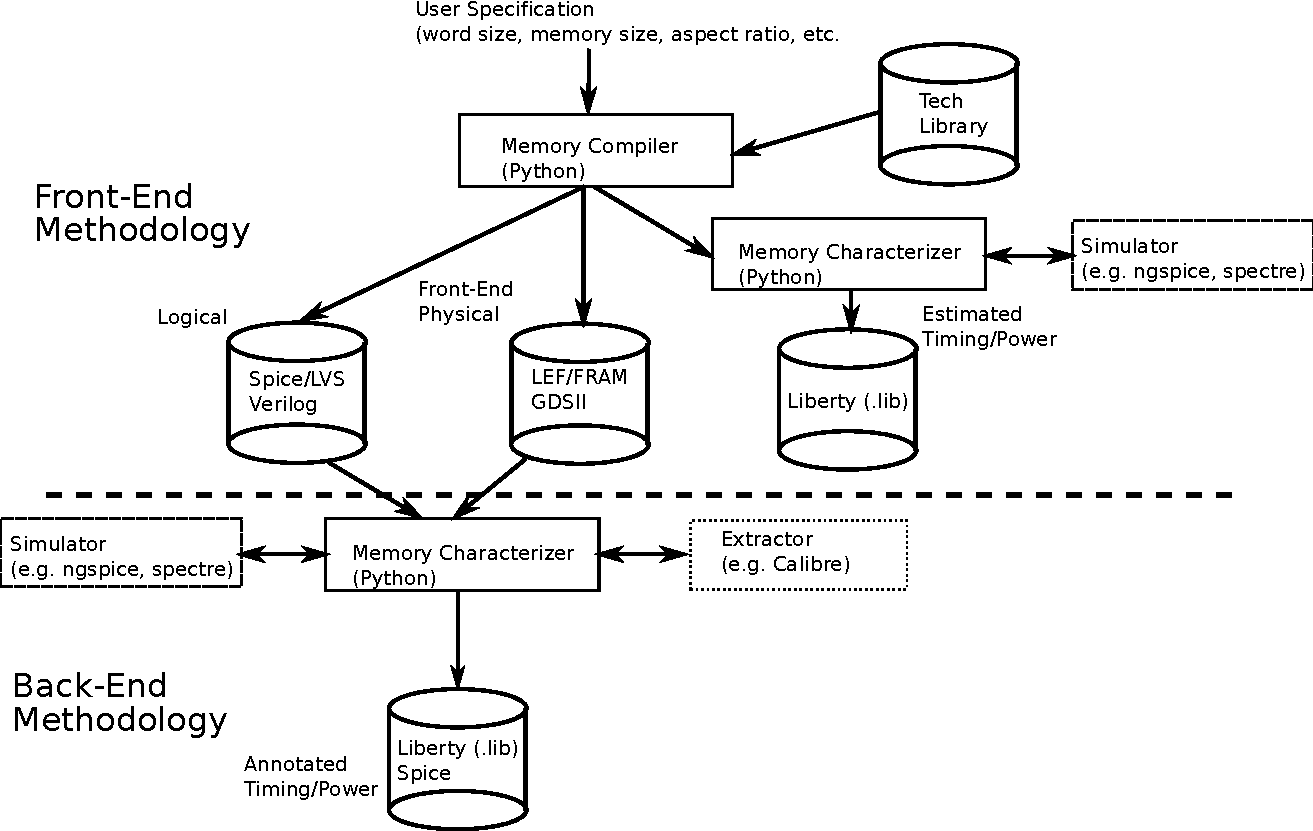
\includegraphics[width=14cm]{./figs/methodology.pdf}
\caption{Overall Compilation and Characterization Methodology
\label{fig:methodology}}
\end{figure}








%%%%%%%%%%%%%%%%%%%%%%%%%%%%%%%%%%%%%%%%%%%%%%%%%%%%%%%%%%%%%%%%%%%%%%%%%%%
\section{Overview of the SRAM Structure}
\label{sec:overview}


% address decode and mem array
The baseline SRAMs generated by OpenRAM have 1 read/write port as
shown in Figure~\ref{fig:sram_architecture}. The address is decoded
(Section~\ref{sec:addressdecoder}) into a one-hot set of word lines
(WL) which are driven by word line drivers
(Section~\ref{sec:wldriver}) over the bit-cell array
(Section~\ref{sec:bitcellarray}). To facilitate reads, the precharge
circuitry (Section~\ref{sec:precharge}) precharges the bitlines so
that the column mux (Section~\ref{sec:column_mux}) can select the
appropriate word which is then sensed by the sense amplifiers
(Section~\ref{sec:senseamp}).  Write drivers
(Section~\ref{sec:writedriver}) use the bidirectional nature of the
column mux to write the appropriate columns in a given memory row.

A representative layout of such a memory closely resembles the logical
representation and is shown in Figure~\ref{fig:layout_view}.  The
address and data flip-flops and control circuitry are not shown but
are detailed in Section~\ref{sec:control}.


\begin{figure}[htb]
\centering
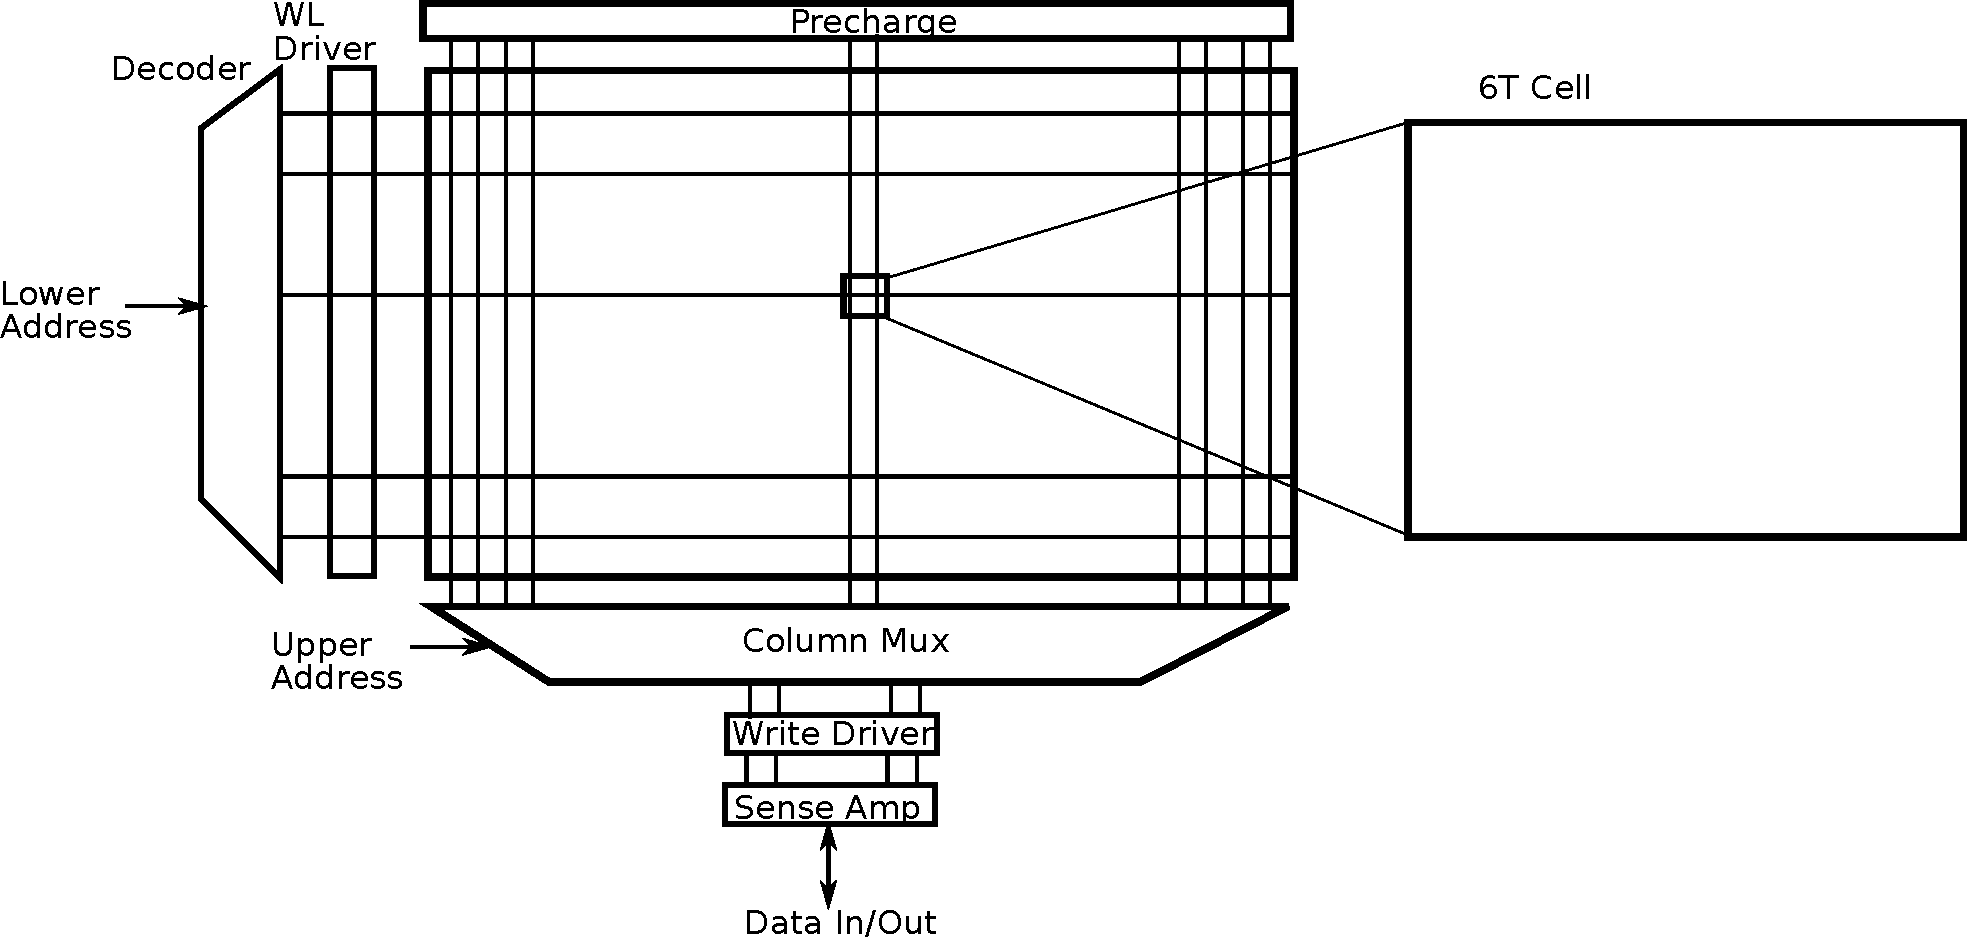
\includegraphics[width=10cm]{./figs/sram_overview.pdf}
\caption{Single Port SRAM Architecture}
\label{fig:sram_architecture}
\end{figure}


\begin{figure}[htb]
\centering
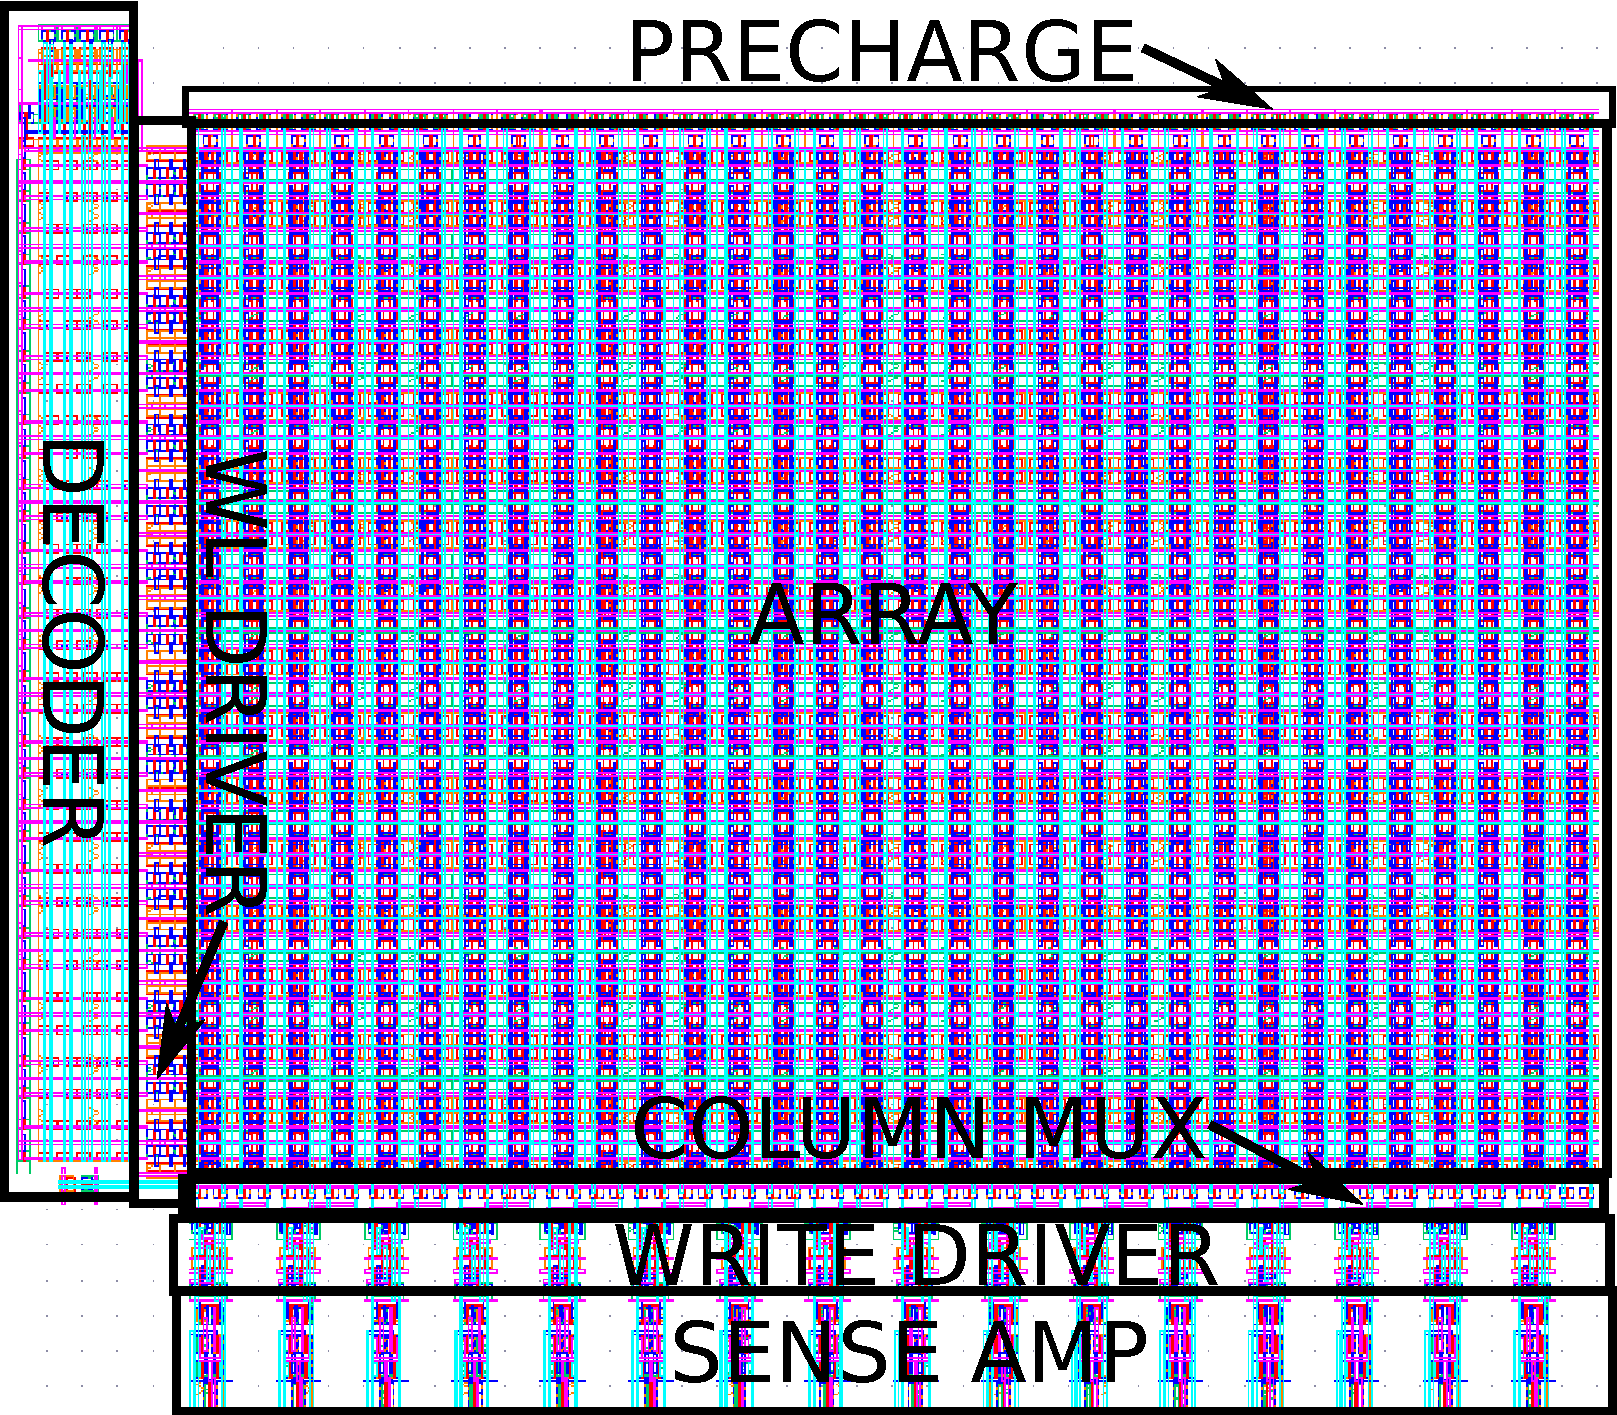
\includegraphics[width=6cm]{./figs/layout_view_1024_16_annotated.pdf}
\caption{1k SRAM with Two Columns and 16-bit Data}
\label{fig:layout_view}
\end{figure}



\subsection{Inputs/Outputs}
\label{sec:io}

The inputs to the SRAM are: 
\begin{itemize}
\setlength{\itemsep}{0pt}
\item clk - External Clock
\item CSb - Active-low Chip Select
\item WEb - Active-low Write Enable
\item OEb - Active-low Output Enable
\item ADDR[\#] - Address Bus input (LSB is 0)
\item DATA[\#] - Bi-directional Data bus (LBS is 0)
\end{itemize}
If multiple ports are used, the ADDR and DATA buses are appended with
integers to extend them.

The outputs to the SRAM are: 
\begin{itemize}
\setlength{\itemsep}{0pt}
\item DATA\# - correspond to the bi-directional Data bus.
\end{itemize}

The supply voltages to the SRAM are:
\begin{itemize}
\item vdd - Supply voltage
\item gnd - Ground supply voltage
\end{itemize}

\subsection{Top-Level SRAM Module}
\label{sec:sram}

The sram class in \verb|sram.py| is the top-level SRAM module.  This
class handles the overall organization of the memory, instantiates the
contorl logic, instantiates a number of banks, and creates decoded
enable signals for multiple banks. All of the top level routing is
performed in the sram class.


The sram class instantiates identical copies of the bank module from
\verb|bank.py|.  All other sub-modules access the value of sizes from
bank.  The bank module includes an address decoder, (optional) column
address decoder, (optional) column mux, sense amplifiers, precharge
circuitry, write drivers, etc.  A single bank organization is depicted
in Figure~\ref{fig:sram_architecture}.

Discussion of the design data structure is discussed in
Section~\ref{sec:design} and the modules contained in the top-level
SRAM are detailed in Section~\ref{sec:modules}.



%%%%%%%%%%%%%%%%%%%%%%%%%%%%%%%%%%%%%%%%%%%%%%%%%%%%%%%%%%%%%%%%%%%%%%%%%%%
\section{Modules}
\label{sec:modules}

This section provides an overview of the main modules that are used in
an SRAM.  For each module, we will provide both an architectural
description and an explanation of how that design is generated and
used in OpenRAM.  The modules described below are provided in the
first release of OpenRAM, but by no means is this an exhaustive list
of the possible circuits that can be adapted into a SRAM architecture;
refer to Section~\ref{sec:implementation} for more information on
adding different module designs to the compiler.

Data structures for schematic and layout are provided in the
\verb|base| directory. These implement a generic design object and
have many auxiliary functions for routing, pin access, placement,
DRC/LVS, etc.  These are discussed further in
Section~\ref{sec:implementation}.

Each module has a corresponding Python class in the
\verb|compiler/modules| directory.  These classes are used to generate
both the GDSII layout and spice netlists. A module can consist of
hard library cells (Section~\ref{sec:techdir}), paramterized
cells (Section~\ref{sec:parameterized}) or other modules.

When combining modules at any level of hierarchy, DRC rules for
minimum spacing of metals, wells, etc. must be followed and DRC and
LVS are run by default after each hierarchical module's creation. A
module is responsible for creating its own pins to enable routing
at the next level up in the hierarchy. A module must also define its
height and width assuming a (0,0) offset for the lower-left coordinate
to aid with placement.


\subsection{The Bitcell and Bitcell Array}
\label{sec:bitcellarray}

OpenRAM can work with any cell as the bitcell. This could be a foundry
created one or a user design rule cell for experiments.  In addition,
it could be a common 6T cell or it could be replaced with an 8T, 10T
or other cell, depending on needs.

By default, OpenRAM uses a standard 6T cell as shown in 
Figure~\ref{fig:6t_cell}.  The cross coupled inverters hold a single
data bit that can either be driven into, or read from the cell by the
bitlines.  The access transistors are used to isolate the cell from
the bitlines so that data is not corrupted while a cell is not being
accessed.

\begin{figure}[h!]
\centering
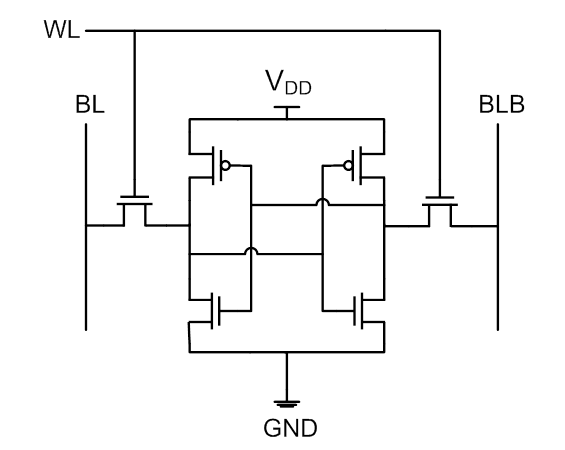
\includegraphics[scale=.9]{figs/cell_6t_schem.pdf}
\caption{Standard 6T cell.}
\label{fig:6t_cell}
\end{figure}

% tiling memory cells
The 6T cells are tiled together in both the horizontal and vertical
directions to make up the memory array.  

% keeping it square
It is common practice to keep the aspect ratio of a memory array
roughly ``square'' to ensure that the bitlines and wordlines do not
become too long. If the bitlines are too long, this can increase the
bitline capacitance, slow down the operation and lead to bitline
leakage problems.  To make an array ``more square'', multiple words
can share rows by interleaving the bits of each word. The column mux
in Section~\ref{sec:column_mux} is responsbile for selecting a subset
of bitcells in a row to extract a word during read and write
operations.

% memory cell is a library cell
In OpenRAM, we provide a library cell for the 6T cell that can be
swapped with a fab memory cell, if available. The transitors in the
cell are sized appropriately considering read and write noise margins.

% bitcell and bitcell_array classes
The bitcell class in \verb|modules/bitcell.py| is a single
memory cell and is usually a pre-made library cell.

% bitcell_array
The bitcell\_array class in \verb|modules/bitcell_array.py| dynamically
implements the memory cell array by instantiating a the bitcell class
in rows and columns.

% abutment connections
During the tiling process, bitcells are abutted so that all bitlines
and word lines are connected in the vertical and horizontal directions
respectively. This is done by using the boundary layer to define the
height and width of the cell. If this is not specified, OpenRAM will
use the bounding box of all shapes as the boundary. The boundary layer
should be offset at (0,0) in the lower left coordinate.

% flipping
In order to share supply rails, bitcells are flipped in alternating
rows. 



\subsection{Precharge Circuitry}
\label{sec:precharge}

The precharge circuit is depicted in Figure~\ref{fig:precharge} and is
implemented by three PMOS transistors. The input signal to the cell,
clk, enables all three transistors during the first half of a read or
write cycle (i.e. while the clock signal is low).  M1 and M2 charge bl
and br to vdd while M3 equalizes the voltages seen between the bitlines.

\begin{figure}[h!]
\centering
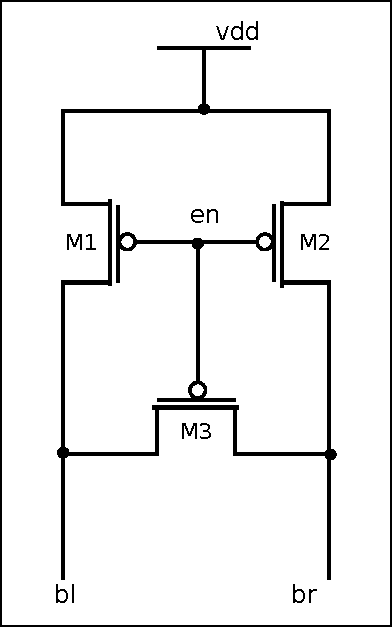
\includegraphics[width=5cm]{./figs/precharge_schem.pdf}
\caption{Schematic of a precharge circuit.}
\label{fig:precharge}
\end{figure}

In OpenRAM, the precharge citcuitry is dynamically generated using the
parameterized transistor class ptx which is further discussed in
Section~\ref{sec:ptx}. The offsets of the bitlines and the width of
the precharge cell are equal to the bitcell so that the bitlines are
correctly connected by abutment. The precharge class in
\verb|modules/precharge.py| dynamically generates a single precharge
cell.

\verb|modules/precharge_array.py| creates a row of precharge cells at
the top of a bitcell array.




\subsection{Address Decoders}
\label{sec:address_decoder}

The address decoder deodes the binary-encoded row address bits from the
address bus as inputs, and asserts a one-hot wordline in the row that
data is to be read or written. OpenRAM provides a hierarchical address
decoder as the default, but will soon have other options.

The address decoders are created using parameterized gates (pnand2,
pnand3, pinv) and transistors (ptx). This means that the decoders do
not rely on any hard library cells.

\subsubsection{Hierarchical Decoder}
\label{sec:hierdecoder}


A simple 2:4 decoder is shown in Figure~\ref{fig:2:4decoder}. This
decoder computes all of the possible decode values using a single
level of nand gates along with the inverted and non-inverted inputs.
As the decoder size increases the size of the nand gates required for
decoding would increase proportional to the bits to be decoded.  This
would not be practical for large decoders.


\begin{figure}[h!]
\centering
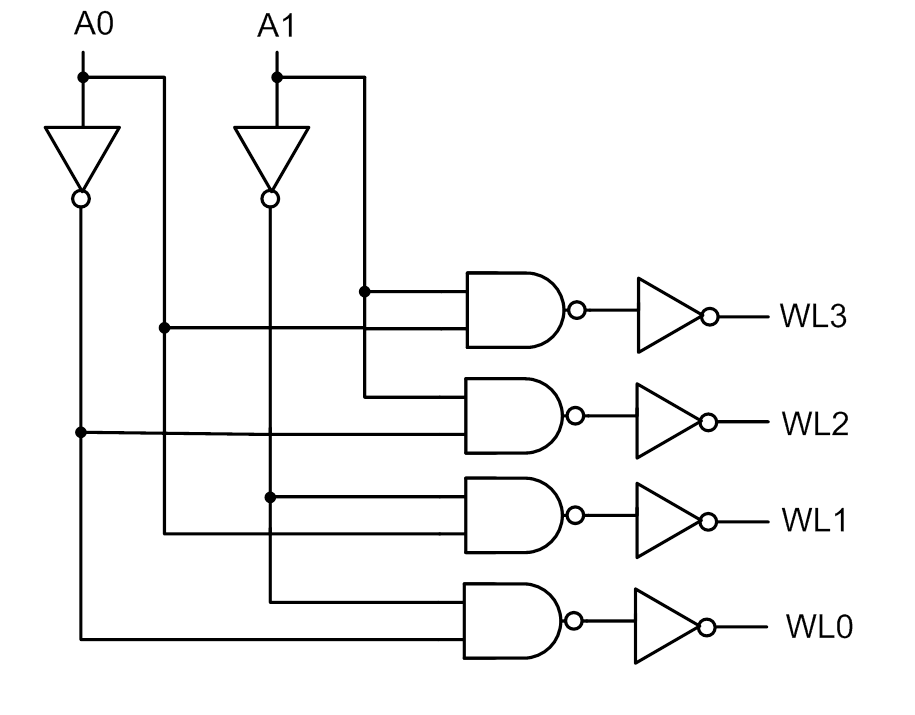
\includegraphics[scale=.6]{./figs/2t4decoder.pdf}
\caption{Schematic of 2-4 simple decoder.}
\label{fig:2:4decoder}
\end{figure}

A hierarchical decoder uses two-levels of decoding hierarchy to
perform an address decode. The first stage computes predecoded values
while the second stage computes the final decoded values.
Figure~\ref{fig:4 to 16 decoder} shows a 4:16 heirarchical
decoder. The decoder uses two 2:4 decoders for
predecoding and 2-input nand gates and inverters for final decoding to
form the 4:16 decoder.

\begin{figure}[h!]
\centering
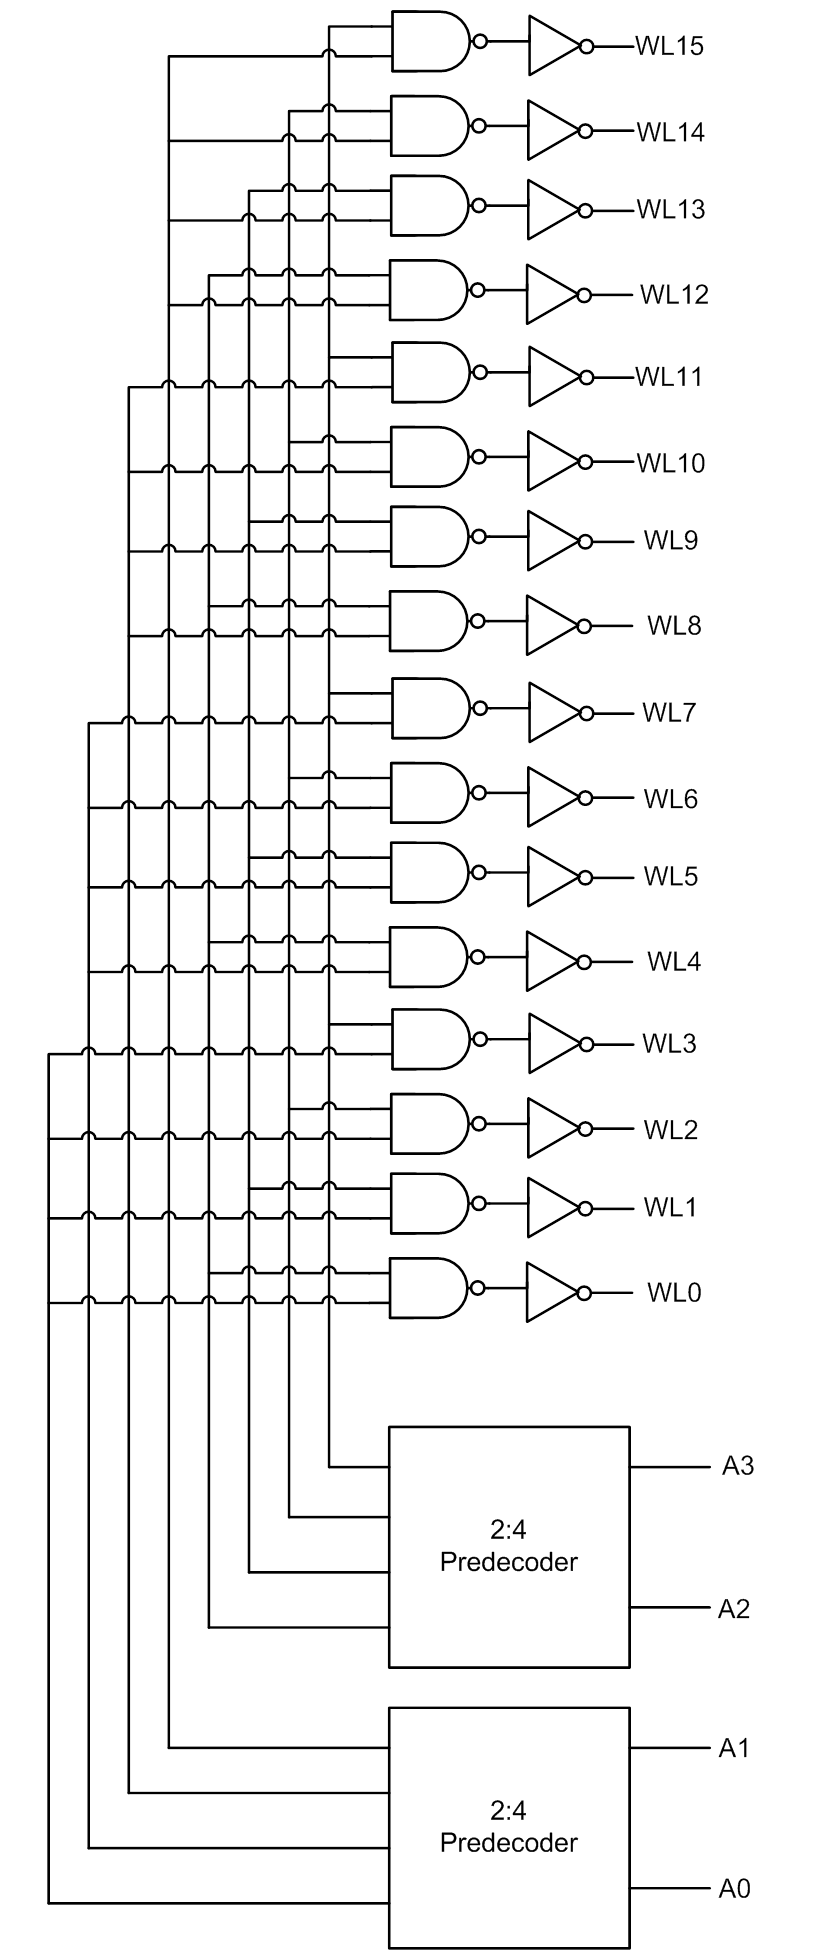
\includegraphics[scale=.6]{./figs/4t16decoder.pdf}
\caption{Schematic of 4:16 hierarchical decoder.}
\label{fig:4 to 16 decoder}
\end{figure}

The predecoder generates a total of 8 intermediate signals from the
address bits and their complements. These intermediate signals are in
two groups of 4 from each decoder. The enumeration of all 4 x 4
predecoded values are used by the final decode to produce the 16
decoded results.  As an example, Table~\ref{table:4-16 hierarchical_decoder}
gives the detailed input and output siganls for the 4:16 hierarchical
decoder.


 \begin{table}[h!] 
   \begin{center}
     \begin{tabular}{| c | c | c | c |}
     \hline
     A[3:0] & predecoder1 & predecoder2 & Selected WL\\ \hline
     0000 & 1000 & 1000 & 0\\ \hline
     0001 & 1000 & 0100 & 1\\ \hline
     0010 & 1000 & 0010 & 2\\ \hline
     0011 & 1000 & 0001 & 3\\ \hline
     0100 & 0100 & 1000 & 4\\ \hline
     0101 & 0100 & 0100 & 5\\ \hline
     0110 & 0100 & 0010 & 6\\ \hline
     0111 & 0100 & 0001 & 7\\ \hline
     1000 & 0010 & 1000 & 8\\ \hline
     1001 & 0010 & 0100 & 9\\ \hline
     1010 & 0010 & 0010 & 10\\ \hline
     1011 & 0010 & 0001 & 11\\ \hline
     1100 & 0001 & 1000 & 12\\ \hline
     1101 & 0001 & 0100 & 13\\ \hline
     1110 & 0001 & 0010 & 14\\ \hline
     1111 & 0001 & 0001 & 15\\ \hline
     \end{tabular}
   \end{center}
   \caption{Truth table for 4:16 hierarchical decoder.}
   \label{table:4-16 hierarchical_decoder}
 \end{table}


As the address size increases, additional sizes of pre- and final
decoders can be used.  In OpenRAM, there are implementations for
\verb|modules/hierarchical\_predecode2x4.py| and
\verb|modules/hierarchical\_predecode3x8.py| to produce 2:4 and 3:8
predecodes, respectively. These same decoders are used to generate the
column mux select bits as well.

For the final decode, we can use either pnand2 or pnand3 gates. This
allows a maximum size of three 3:8 predocers along with a final pnand3 decode
stage, or, 512 word lines. To extend beyond this, a pnand4 or
a 4:16 predecoder would be needed.


\subsection{Wordline Driver}
\label{sec:wldriver}

The word line driver buffers the address decoder to drive the wordline and
gates the signal until the decode has stabilized. Without waiting, an
incorrectly asserted wordline could erase memory contents.
The word line driver is sized according to the bitcell array width so
that wordlines in larger memory arrays can be appropriately driven.

% gating for first half decode, second half read/write
The first half of the clock cycle is used for address decoding in
OpenRAM.  Therefore, the wordline driver is enabled in the second half
of the clock cycle in OpenRAM.  The buffered clock signal drives each
wordline driver row and is logically ANDed with the decoder output.

% bank clock gating for wordline driver
In multi-bank structures the clock buffer is also anded with the bank
select signal to prevent the read/writing of an entire bank.

\begin{figure}[h!]
\centering
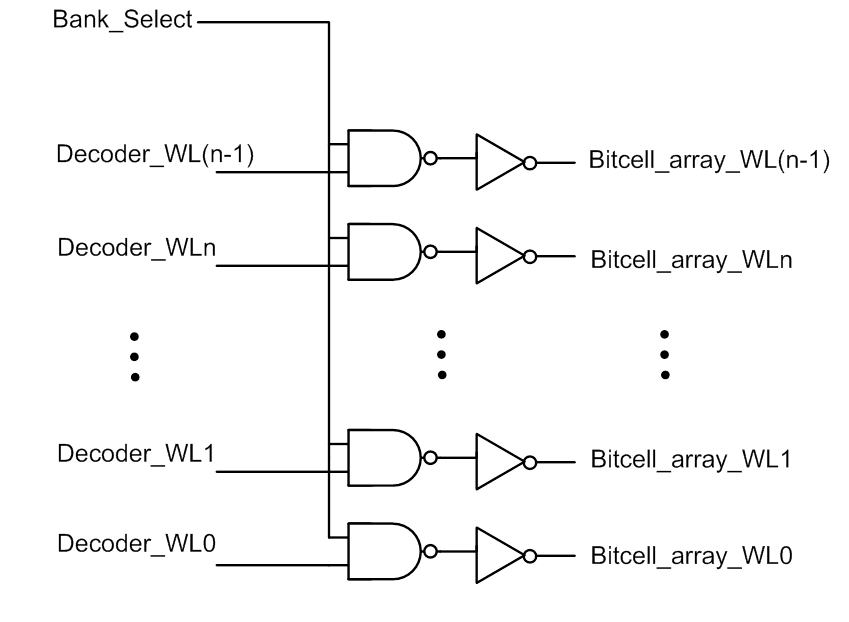
\includegraphics[scale=.6]{./figs/wordline_driver.pdf}
\caption{Diagram of word line driver.}
\label{fig:wordline_driver}
\end{figure}

Figure~\ref{fig:wordline_driver} illustrates the wordline driver and
its inputs/outputs. This is implemented in the
\verb|modules/wordline_driver.py| module and matches the number of
rows in the bitcell array of a bank.

OpenRAM creates the wordline drivers using the parameterized pinv and
pnand2 classes. This enables the wordline driver to be matched to the
bitcell height and to sized to drive the wordline load.



\subsection{Column Mux}
\label{sec:column_mux}
The column mux is an optional module in an SRAM bank. Without a column
mux, the bank is assumed to have a single word in each row. A column
mux enables more more than one word to be stored in each row and
read/written individually.  The column mux is used for both the read
and write operations by connecting the bitlines of a bank to
both the sense amplifier and the write driver.

In OpenRAM, the column mux uses the {\bf high address bits} to select
the appropriate word in each row.  If n-bits are used, there are $2^n$
words in each row. OpenRAM currently allows 2, 4, or 8 words per row,
but the 8 words are not fully debugged (as of 2/12/18).

%% OpenRAM provides several options for column mux, but the default
%% is a single-level column mux which is sized for optimal speed.

%% \subsubsection{Tree\_Decoding Column Mux}
%% \label{sec:tree_decoding_column_mux}

%% The schematic for a 4-1 tree
%% multiplexer is shown in Figure~\ref{fig:colmux}.

%% \begin{figure}[h!]
%% \centering
%% 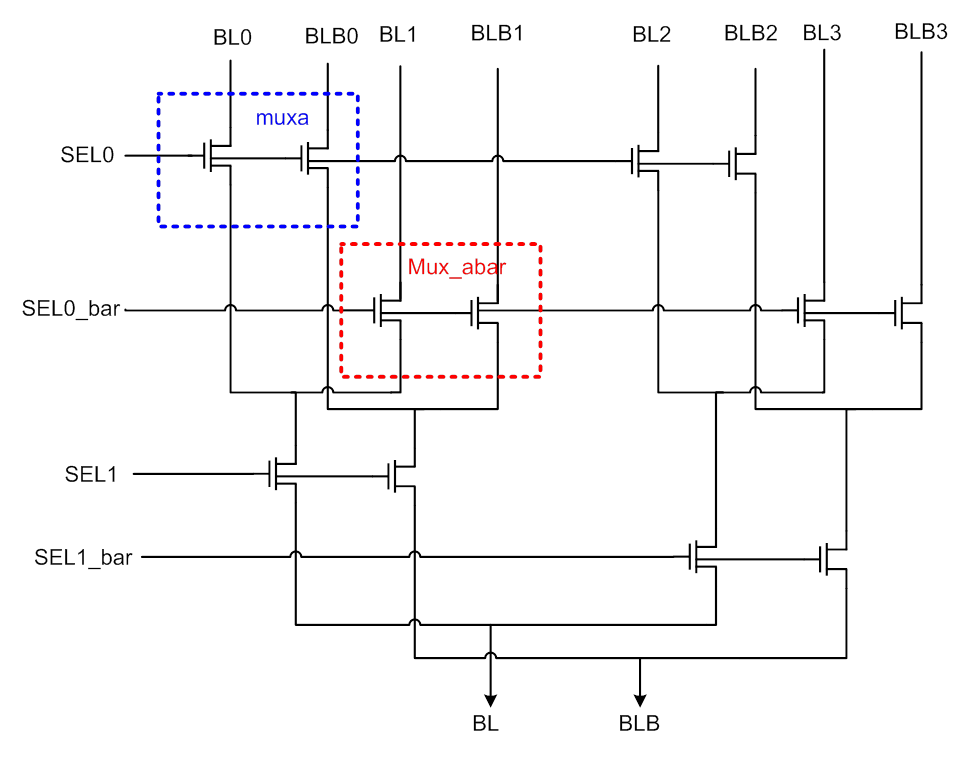
\includegraphics[scale=.9]{./figs/tree_column_mux_schem.pdf}
%% \caption{Schematic of 4-1 tree column mux that passes both of the bitlines.}
%% \label{fig:colmux}
%% \end{figure}

%% \fixme{Shading/opacity is different on different platforms. Make this a box in the image. It doesn't work on OSX.}

%% This tree mux selects pairs of bitlines (both BL and BL\_B) as inputs
%% and outputs.  This 4-1 tree mux illustrates the process of choosing
%% the correct bitlines if there are 4 words per row in the memory array.
%% Each bitline pair represents a single bit from each word.  A binary
%% reduction pattern, shown in Table~\ref{table:colmux}, is used to
%% select the appropriate bitlines.  As the number of words per row in
%% the memory array increases, the depth of the column mux grows.  The
%% depth of the column mux is equal to the number of bits in the column
%% address bus.  The 4-1 tree mux has a depth of 2.  In level 1, the
%% least significant bit from the column address bus selects either the
%% first and second words or the third and fourth words.  In level 2, the
%% most signifant column address bit selects one of the words passed down
%% from the previous level.  Relative to other column mux designs, the
%% tree mus uses significantly less devices.  But, this type of design
%% can provide poor performance if a large decoder with many levels are
%% needed.  The delay of of a tree mux quadratically increases with each
%% level.  Due to this fact, other types of column
%% decoders should be considered for larger arrays.

%% \begin{table}[h!] 
%%   \begin{center}
%%     \begin{tabular}{| c | c | c | c |}
%%     \hline
%%     Selected BL & Inp1 & Inp2 & Binary\\ \hline
%%     BL0 & SEL0\_bar & SEL1\_bar & 00\\ \hline
%%     BL1 & SEL0 & SEL1\_bar & 01\\ \hline
%%     BL2 & SEL0\_bar & SEL1 & 10\\ \hline
%%     BL3 & SEL0 & SEL1 & 11\\
%%     \hline
%%     \end{tabular}
%%   \end{center}
%%   \caption{Binary reduction pattern for 4-1 tree column mux.}
%%   \label{table:colmux}
%% \end{table} 

%% In OpenRAM, the tree column mux is a dynamically generated design.  The
%% \verb|tree_mux_array| is made up of two dynamically generated cells: \verb|muxa|
%% and \verb|mux_abar|.  The only diffference between these cells is that input
%% select signal is either hooked up to the \textbf{SEL} or
%% \textbf{SEL\_bar} signals (see highlighted boxes in
%% Figure~\ref{fig:colmux}).  These cells are initialized the the
%% \verb|column_muxa| and \verb|column_muxabar| classes in \verb|columm_mux.py|.  Instances
%% of \verb|ptx| PMOS transistors are added to the design and the necessary
%% routing is performed using the \verb|add_rect()| function. A horizontal rail
%% is added in metal2 for both the SEL and Sel\_bar signals.  Underneath
%% those input rails, horizontal straps are added.  These straps are used
%% to connect the BL and BL\_B outputs from \verb|muxa| to the BL and BL\_B
%% outputs of \verb|mux_abar|.  Vertical conenctors in metal3 are added at the
%% bottom of the cell so that connections can be made down to the sense
%% amp.  Vertical connectors are also added in metal1 so that the cells
%% can connect down to other mux cells when the depth of the tree mux is
%% more than one level.

%% The \verb|tree_mux_array| class is used to generate the tree mux.
%% Instances of both the \verb|muxa| and \verb|mux_abar| cells are instantiated and
%% are tiled row by row.  The offset of the cell in a row is determined
%% by the depth of that row in the tree mux.  The pattern used to
%% determine the offset of the mux cells is
%% $muxa.width*(i)*(2*row\_depth)$ where is the column number.  As the
%% depth increases, the mux cells become further apart.  A separate
%% ``for'' loop is invoked if the $depth>1$, which extends the
%% power/ground and select rails across the entire width of the array.
%% Similarly, if the $depth>1$, spice net names are created for the
%% intermediate connection made at the various levels.  This is necessary
%% to ensure that a correct spice netlist is generated and that the
%% input/output pins of the column mux match the pins in the modules that
%% it is connected to.


\subsubsection{Single-Level Column Mux}
\label{sec:single_level_column_mux}

OpenRAM includes a single-level pass-gate mux implemtation for the
column mux.  A single level of NMOS devices is driven by either the
input address (and it's complement) or decoded input addresses using a
2:4 predecoder (Section~\ref{sec:hierdecoder}).

Figure~\ref{fig:2t1_single_level_column_mux} shows the schematic of a
2:1 single-level column mux. In this column mux, the {\bf MSB of the
  address bus} and it's complement drive the pass transistors.

Figure~\ref{fig:4t1_single_level_column_mux} shows the schematic of a
4:1 single-level column mux. The select bits are decoded from the {\bf
  2 MSB of the address bus} using a 2:4 decoder.  The 2:4 decoder
provides one-hot select signals to select one column.

In OpenRAM, one mux, single\_level\_mux, is dynamically generated in
\verb|modules/single_level_column_mux.py| and multiple of these muxes
are tiled together in \verb|modules/single_level_column_mux_array.py|.

single\_level\_mux uses the parameterized ptx (Section~\ref{sec:ptx}
to generate 2 or 4 NMOS transistors for each the bl and br
bitlines. Horizontal rails are added for the $sel$ signals.  The
bitlines are automatically pitch-matched to the bitcell array.


\begin{figure}[h!]
\centering
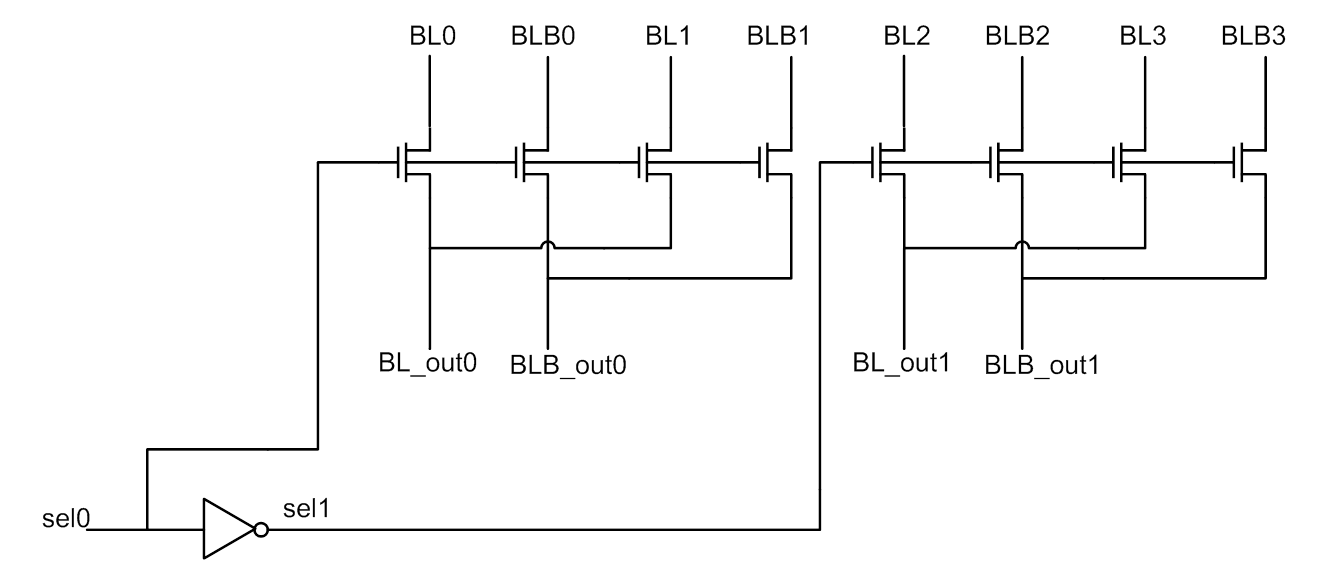
\includegraphics[scale=.5]{./figs/2t1_single_level_column_mux.pdf}
\caption{Schematic of a 2:1 single level column mux. \fixme{Signals names are wrong.}}
\label{fig:2t1_single_level_column_mux}
\end{figure}



\begin{figure}[h!]
\centering
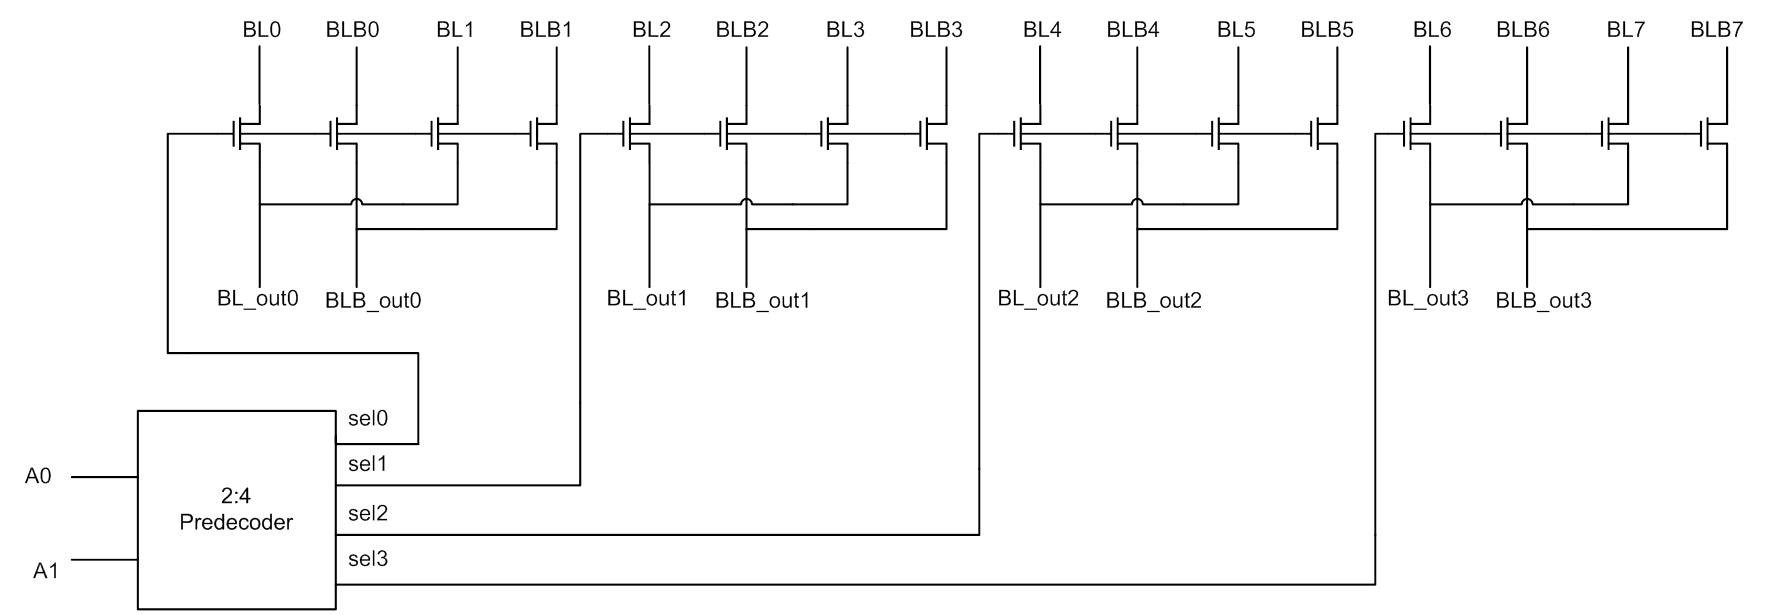
\includegraphics[scale=.5]{./figs/4t1_single_level_column_mux.pdf}
\caption{Schematic of a 4:1 single level column mux. \fixme{Signals names are wrong.}}
\label{fig:4t1_single_level_column_mux}
\end{figure}


\subsection{Sense Amplifier}
\label{sec:senseamp}
The sense amplifier is used to sense the difference between the
bitline and bitline bar while a read operation is performed.  The
sense amp is necessary to recover the signals from the bitlines
because they do not experience full voltage swing.  As the size of the
memory array grows, the load of the bitlines increases and the voltage
swing is limited by the small memory cell driving this large load.  A
differential sense amplifier is used to``sense'' the small voltage
difference between the bitlines.

\begin{figure}[h!]
\centering
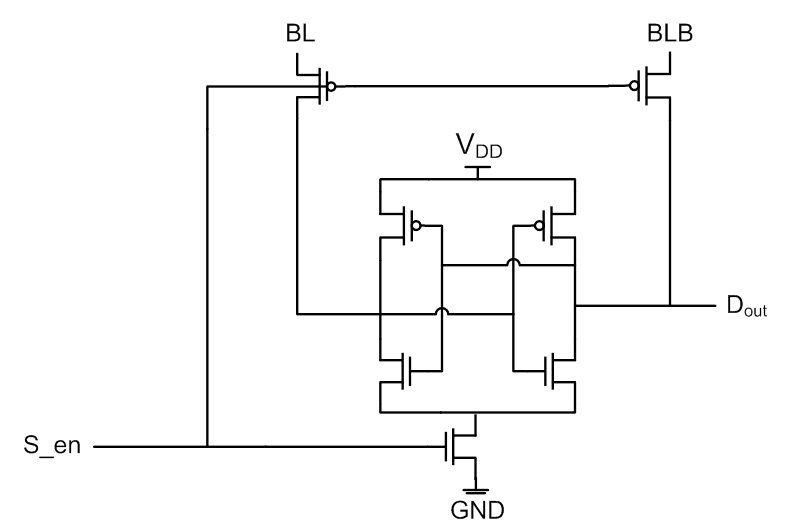
\includegraphics[scale=.8]{./figs/sense_amp_schem.pdf}
\caption{Schematic of a single sense amplifier cell.}
\label{fig:sense_amp}
\end{figure}

The schematic for the sense amp is shown in
Figure~\ref{fig:sense_amp}.  The sense amplifier is enable by the SCLK
signal, which initiates the read operation.  Before the sense
amplifier is enable, the bitlines are precharged to Vdd by the
precharge unit.  When the sense amp is enabled, one of the bitlines
experiences a voltage drop based on the value stored in the memory
cell.  If a zero is stored, the bitline voltage drops.  If a one is
stored, the bitline bar voltage drops.  The output signal is then
taken to a true logic level and latched for output to the data bus.

In OpenRAM, the sense amplifier is a libray cell.  The associated
layout and spice netlist can be found in the \verb|gds_lib| and \verb|sp_lib| in
the FreePDK45 directory.  The \verb|sense_amp| class in \verb|sense_amp.py|
instantiates a single instance of the sense amp library cell.  The
\verb|sense_amp_array| class handles the tiling of the sense amps cells.
One sense amp cell is needed per data bit and the sense amp cells need
to be appropriately spaced so that they can hook up to the column mux
bitline pairs.  The spacing is determined based on the number of words
per row in the memory array.  Instances are added and then Vdd, Gnd
and SCLK rails that span the entire width of the array are drawn using
the add\_rect() function.

We chose to leave the sense amp as a libray cell so that custom
amplifier designs could be swapped into the memory as needed.  The two
major things that need to be considered while designing the sense
amplifier cell are the size of the cell and the bitline/input pitches.
Optimally, the cell should be no larger than the 6T cell so that it
abuts to the column mux and no extra routing or space is needed.
Also, the bitline inputs of the sense amp need to line up with the
outputs of the write driver.  In the current version of OpenRAM, the
write driver is situated under the sense amp, which had bitlines
spaning the entire height of the cell.  In this case, the sense
amplifier is disabled during a write operation but the bitlines still
connect the write driver to the column mux without any extra routing.


\subsection{Write Driver}
\label{sec:writedriver}
The write driver is used to drive the input signal into the memory
cell during a write operation.  It can be seen in
Figure~\ref{fig:write_driver} that the write driver consists of two
tristate buffers, one inverting and one non-inverting.  It takes in a
data bit, from the data bus, and outputs that value on the bitline,
and its complement on bitline bar.  The bitlines need to be
complements so that the data value can be correctly stored in the 6T
cell. Both tristates are enabled by the EN signal.

\begin{figure}[h!]
\centering
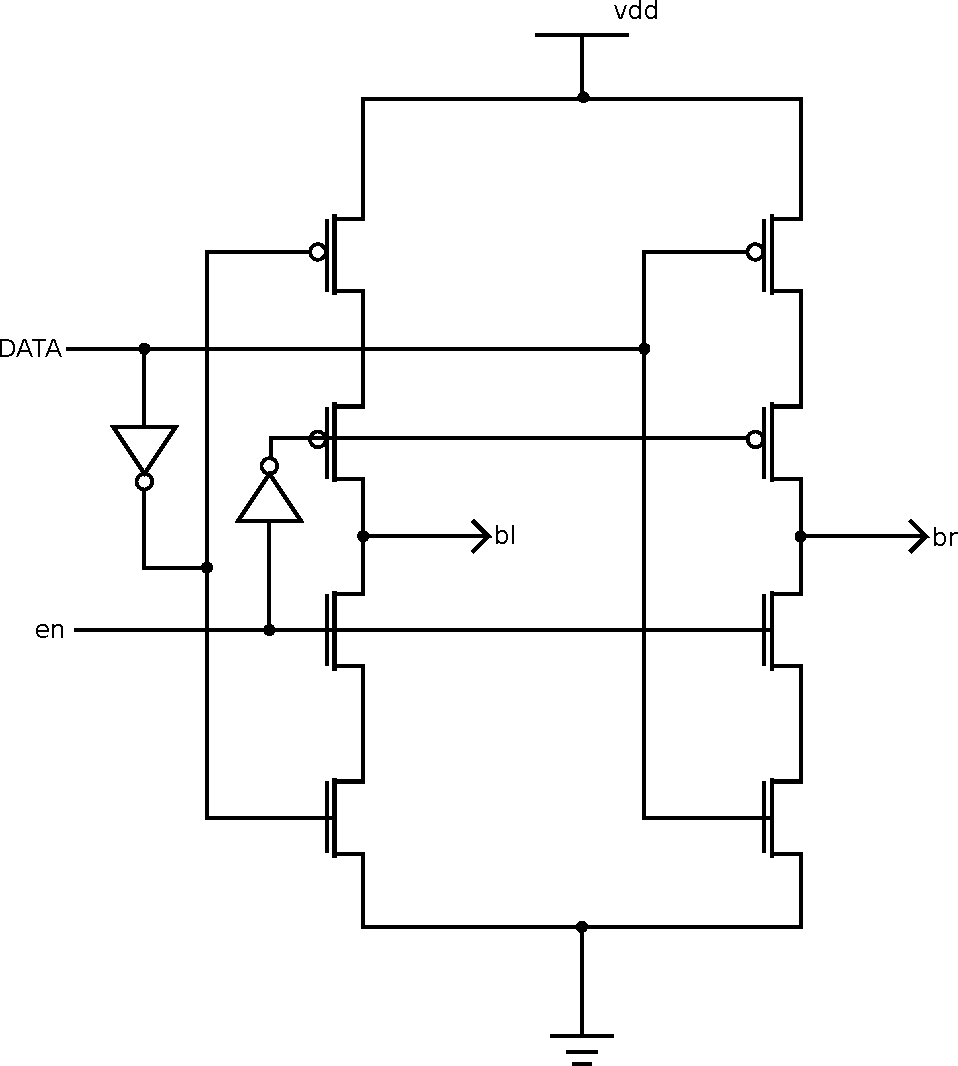
\includegraphics[scale=.8]{./figs/write_driver_schem.pdf}
\caption{Schematic of a write driver cell, which consists of 2 tristates (non-inverting and inverting) to drive the bitlines.}
\label{fig:write_driver}
\end{figure}

Currently, in OpenRAM, the write driver is a library cell.  The
associated layout and spice netlist can be found in the \verb|gds_lib| and
\verb|sp_lib| in the FreePDK45 directory.  Similar to the \verb|sense_amp_array|,
the \verb|write_driver_array| class tiles the write driver cells.  One
driver cell is needed per data bit and Vdd, Gnd, and EN signals must
be extended to span the entire width of the cell. It is not optimal to
have the write driver as a library cell because the driver needs to be
sized based on the capacitance of the bitlines.  A large memory array
needs a stronger driver to drive the data values into the memory
cells.  We are working on creating a parameterized tristate class,
which will dynamically generate write driver cells of different
sizes/strengths.

\subsection{Flip-Flop Array}

In a synchronous SRAM it is necessary to synchronize the inputs and
outputs with a clock signal by using flip-flops.  In FreePDK45 we
provide a library cell for a simple master-slave flip-flop, see
schematic in Figure~\ref{fig:ms_flop}.  In our library cell we provide
both Q and Q\_bar as outputs of the flop because inverted signals are
used in various modules.  The \verb|ms_flop| class in \verb|ms_flop.py|
instatitates a single master-slave flop, and the \verb|ms_flop_array| class
generates an array of flip-flops.  Arrays of flops are necessary for
the data bus (an array for both the inputs and outputs) as well as the
address bus (an array for row and column inputs).  The \verb|ms_flop_array|
takes the number of flops and the type of array as inputs.  Currently,
the type of the array must be either ``data\_in'', ``data\_out'',
``addr\_row'', or ``addr\_col'' verbatim.  The array type input is
used to look up that associated pin names for each of the flop arrays.
This was implemented very quickly and should be improved in the near
future...

\begin{figure}[h!]
\centering
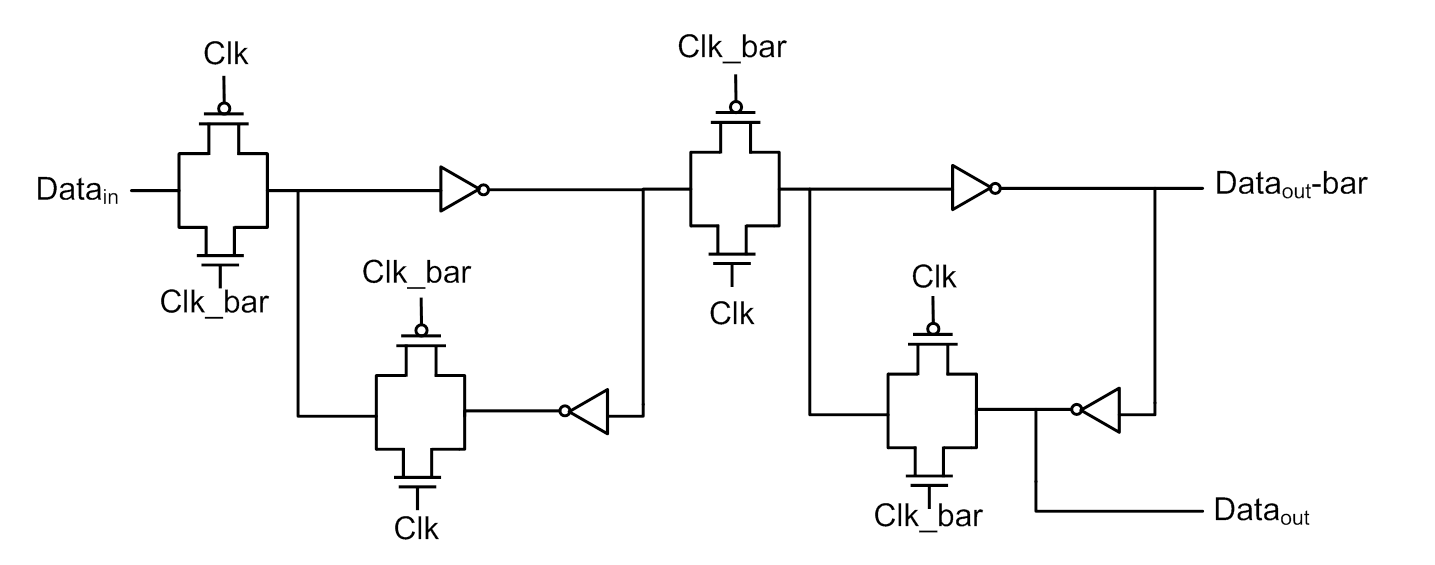
\includegraphics[scale=.7]{./figs/ms_flop_schem.pdf}
\caption{Schematic of a master-slave flip-flop provided in FreePDK45 library}
\label{fig:ms_flop}
\end{figure}

\subsection{Control Logic}

The details of the control logic architecture are outlined in
Section~\ref{sec:control}.  The control logic module,
\verb|control_logic.py|, instantiates a \verb|control_logic| class that arranges
all of the flip-flops and logic associated with the control signals
into a single module. Flip-flops are instantiated for each control
signal input and library NAND and NOR gates are used for the logic.  A
delay chain, of variable length, is also generted using parameterized
inverters.  The associated layouts and spice netlists can be found in
the \verb|gds_lib| and \verb|sp_lib| in the FreePDK45 directory.

\section{Bank and SRAM}
\label{sec:bank}

The overall memory architecture is shown in figure~\ref{fig:bank}.
As shown in this figure one Bank contains different modules including 
precharge-array which is positioned above the bitcell-array, 
column-mux-array which is located below the bitcell-array, 
sense-amp-array, write-driver-array, data-in-ms-flop-array 
to synchronize the input data with negative edge of the clock, 
tri-gata-array to share the bidirectional data-bus between input 
and output data, hierarchical decoder which is placed on the right side 
of the bitcell-array (predecoder + decoder), wordline-driver which drives 
the wordlines horizontally across the bitcell-array and address-ms-flops 
to synchronize the input address with positive edge of the clock. 

In bitcell-array each memory cell is mirrored vertically and horizontally inorder to share VDD and GND rails with adjacent cells and form the array. 
Data-bus is connected to tri-gate, address-bus is connected to address-ms-flops and bank-select 
signal will enable the bank when it goes high. To complete the SRAM design, bank is connected to control-logic as shown in figure~\ref{fig:bank}. 
Control-logic controls the timing 
of modules inside the bank. CSb, OEb, Web and clk are inputs to the control logic and output of 
control logic will ANDed with bank-select signal and send to the corresponding modules.


\begin{figure}[h!]
\centering
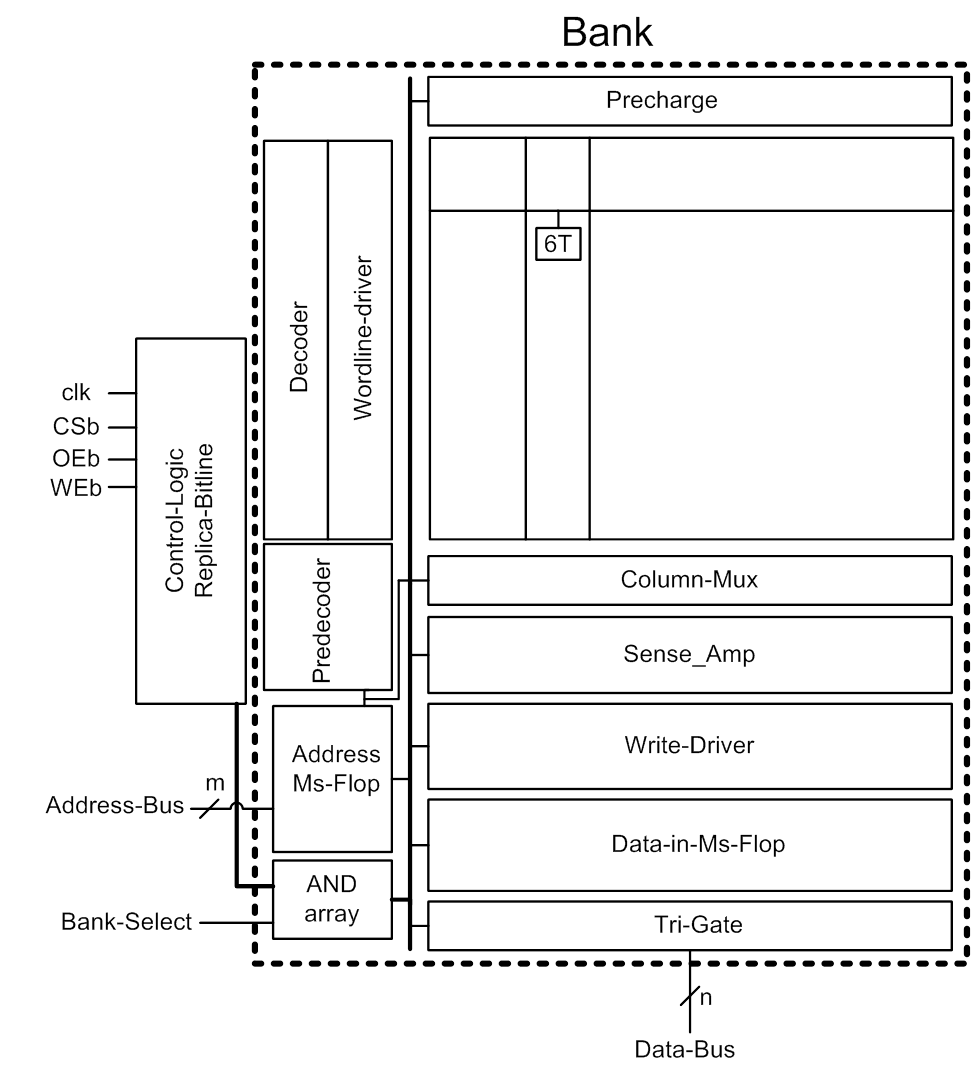
\includegraphics[scale=1]{./figs/bank.pdf}
\caption{Overal bank and SRAM architecture.}
\label{fig:bank}
\end{figure}


In order to reduce the delay and power, divided wordline strategy have been used in this compiler. Part of the address bits 
are used to define the global wordline (bank-select) and rest of address bits are connected to hierarchical 
decoder inside each bank to generate local wordlines that actually drive the bitcell access transistors. 

As shown in figure~\ref{fig:bank2} SRAM is divided to two banks which share data-bus, address-bus, control-bus and control-logic. 
In this case one bit of address (most significant bit) goes to an ms-flop and outputs of ms-flop (address-out and address-out-bar) 
are connected to banks as bank-select signals. Control logic is shared between two banks and based on which bank is selected, 
control signals will activate modules inside the selected bank. In this architecture, the total cell capacitance is reduced by up 
to a factor of two. Therefore the power will be reduced greatly and the delay among the wordlines is also reduced.

\begin{figure}[h!]
\centering
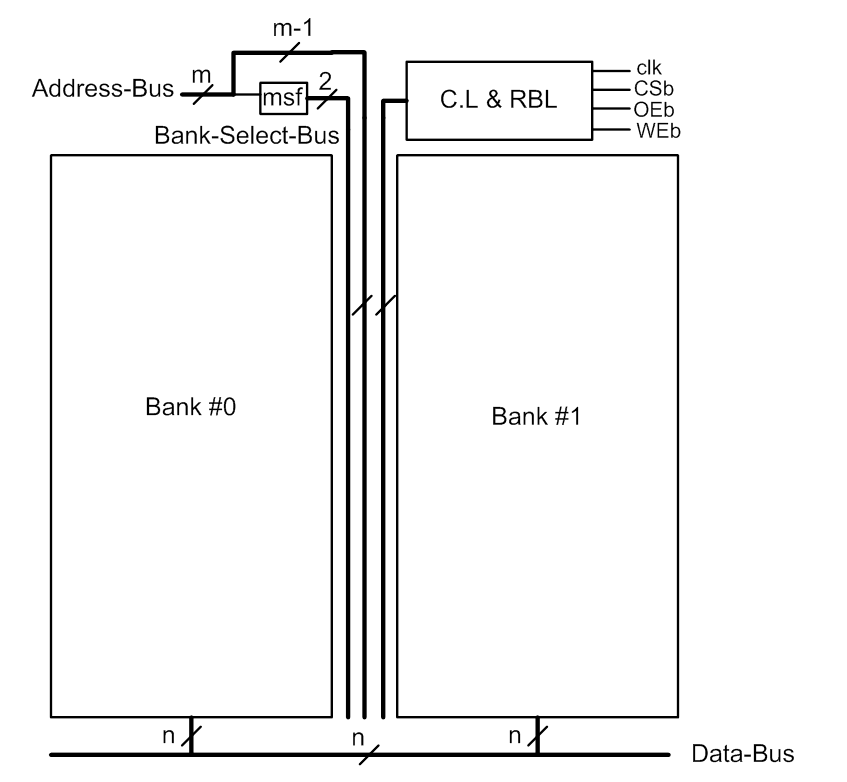
\includegraphics[scale=.9]{./figs/bank2.pdf}
\caption{SRAM is divided to two banks which share the control-logic.}
\label{fig:bank2}
\end{figure}

In figure~\ref{fig:bank4}, four banks are connected together. In this case a 2:4 decoder is added to select one of the banks using two 
most significant bits of input address. Control signals are connected to all banks but will turn on only the selected bank.


\begin{figure}[h!]
\centering
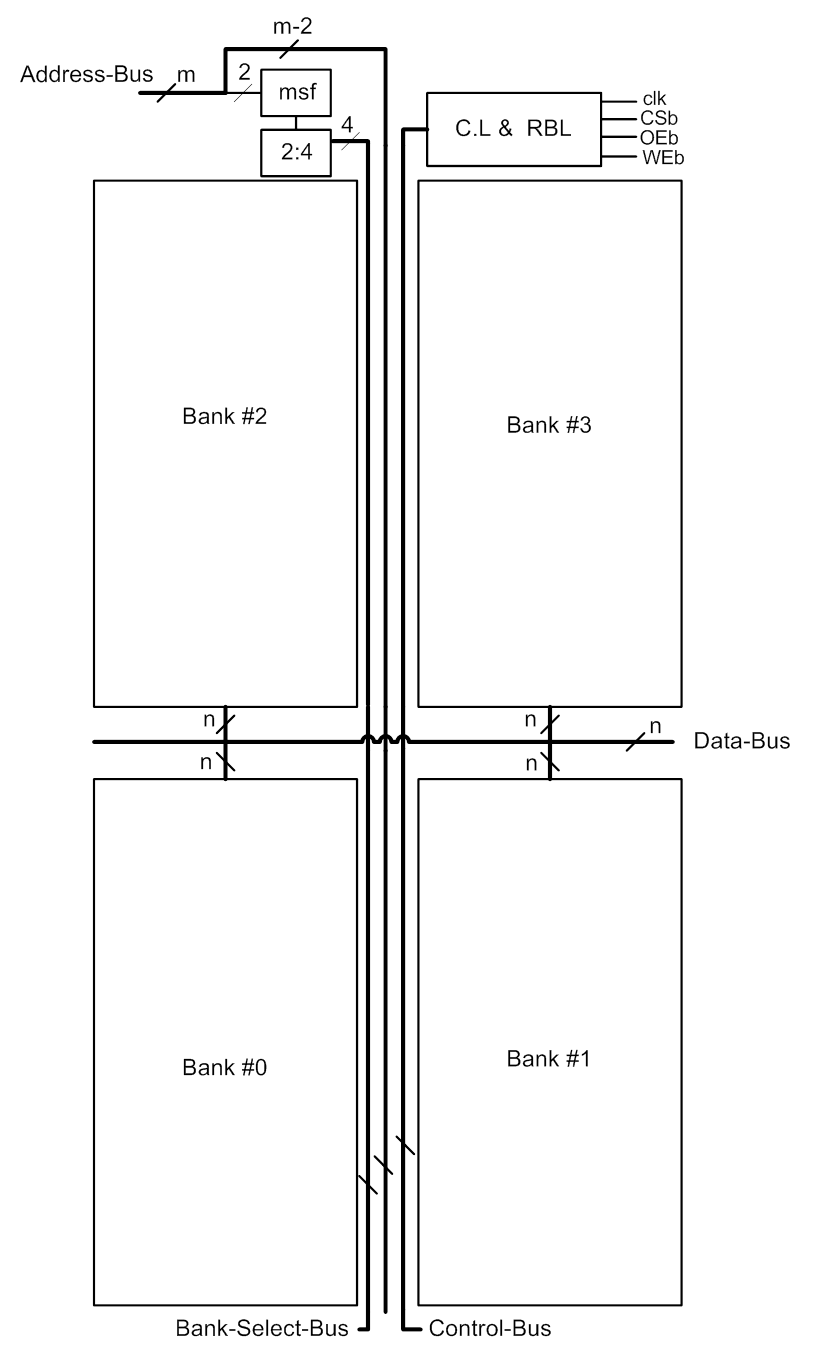
\includegraphics[scale=.9]{./figs/bank4.pdf}
\caption{SRAM is divided to 4 banks wich are controlled by the control-logic and a 2:4 decoder.}
\label{fig:bank4}
\end{figure}




%%%%%%%%%%%%%%%%%%%%%%%%%%%%%%%%%%%%%%%%%%%%%%%%%%%%%%%%%%%%%%%%%%%%%%%%%%%
\section{Software Implementation}
\label{sec:implementation}

OpenRAM is implemented using object-oriented data structures in the
Python programming language. The top-level executable is
\verb|openram.py| which parses input arguments, creates the memory and
saves the output.


\subsection{Design Hierarchy}
\label{sec:design}

All modules in OpenRAM are derived from the \verb|design| class in
\verb|design.py|. The design class is a data structure that consists
of a spice netlist, a layout, and a name. The spice netlist
capabilities are inherited from the \verb|hierarchy_spice| class while
the layout capabilities are inherited from the \verb|hierarchy_layout|
class.  The only additional function in design.py is \verb|DRC_LVS()|,
which performs a DRC/LVS check on the module.


\begin{figure}[htb]
\centering
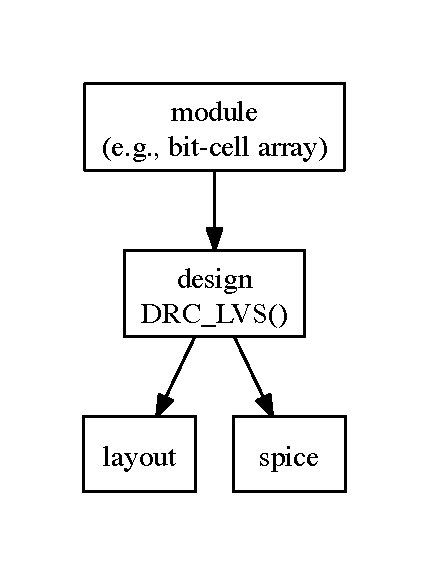
\includegraphics[width=10cm]{./figs/class_hierarchy.pdf}
\caption{Class hierarchy}
\label{fig:class_hierarchy}
\end{figure}

\subsubsection{Spice Hierarchy}

The spice hierarchy is stored in the \verb|spice| class in
\verb|hierarchy_spice.py|.  When the design class is initialized for a
module, a data structure for the spice hierarchy is created.  The
spice data stucture name becomes the name of the top-level subcircuit
definition for the module.  The list of pins for the module are added
to the subcircuit definition by using the \verb|add_pin()| function.
The \verb|add_mod()| function adds an instance of a
module/library\_cell/parameterized\_cell as a subcircuit to the
top-level structure.  Each time a sub-module has been added to the
hierarchy, the pins of the sub-module must be connected using the
\verb|connect_pins()| function.  It is important to note that the pins
must be listed in the same order as they were added to the submodule.
Also, an assertion error will occur if there is a mismatch in the
number of net connections.  The \verb|spice| class also contains
functions for reading or writing spice files:
\begin{itemize}
\item \verb|sp_read():| this function is used to read in spice
  netlists and parse the inputs defined by the ``subckt'' definition.
\item \verb|sp_write():| this function creates an empty spice file in
  write mode and calls \verb|sp_write_file()|.
\item \verb|sp_write_file():| this function recursively writes the
  modules and sub-modules from the data structure into the spice file
  created by \verb|sp_write()|.
\end{itemize}

\subsubsection{Layout Hierarchy}

The layout hierarchy is stroed in the \verb|layout| class in
\verb|hierarchy_layout.py|.  When the design class is initialized for
a module, a data structure for the layout hierarchy is created.  The
layout data structure has two main components: a structure for the
instances of sub-modules contained in the layout, and a structure for
the objects (such as shapes, labels, etc...) contained in the layout.
The functions included in the \verb|layout| class are:
\begin{itemize}
\item \verb|def add_inst(self,name,mod,offset,mirror):| adds an
  instance of a physical layout (library cell, module, or
  parameterized cell) to the module. The input parameters are :
  \begin{description}
  \item[name] - name for the instance.
  \item[mod] - the associated spice module.
  \item[offset] - the x-y coordinates, in microns, where the instance
    should be placed in the layout.
  \item[mirror] - mirror or rotate the instance before it is added to
    the layout.  Accepted values for mirror are:
    \verb|"R0", "R90", "R180", "R270"|  $^\ast$Currently, only ``R0'' works.\\
    \verb|"MX" or "x", "MY" or "y", "XY" or "xy"| (``xy'' is
    equivalent to ``R180'')
  \end{description}
\item \verb|add_rect(self,layerNumber,offset,width,height):| adds a
  rectangle to the module's layout. The inputs are:
  \begin{description}
  \item[layernumber] - the layer that the rectangle is to be drawn in.
  \item[offset] - the x-y coordinates, in microns, where the
    rectangle's origin will be placed in the layout.
  \item[width] - the width of the rectangle, can be positive or
    negative value.
  \item[height] - the height of the rectangle, can be positive or
    negative value.
  \end{description}
\item \verb|add_label(self,text,layerNumber,offset,zoom):| adds a
  label to the layout. The inputs are:
  \begin{description}
  \item[text] - the text for the label
  \item[layernumber] - the layer that the label is to be drawn in .
  \item[offset] - the x-y coordinates, in microns, where the label
    will be placed in the layout.
  \item[zoom] - magnification of the label (ex: ``1e9'').
  \end{description}
\item \verb|add_path(self,layerNumber,coordinates,width):| this
  function is under construction...
\item \verb|gds_read():| reads in a GDSII file and creates a
  \verb|VlsiLayout()| class for it.
\item \verb|gds_write():| writes the entire GDS of the object to a
  file by gdsMill \verb|vlsiLayout()| class and calling the
  \verb|gds2writer()| (see Sections~\ref{sec:vlsilayout}
  and~\ref{sec:gdsmill}.
\item \verb|gds_write_file():| recursively the instances and objects
  in layout data structure to the gds file.
\item \verb|pdf_write():| this function is under construction...
\end{itemize}


\subsection{Creating a New Design Module}
\label{sec:new_design}

Each module in the SRAM is its own Python class, which contains a
design class, or data structure, for the layout and spice.  The
\verb|design| class (\verb|design.py|) is initialized within the
module class, subsequently creating separate data structurse to hold
the layout (\verb|hierarchy_layout|) and spice
(\verb|hierarchy_spice|) information.  By having a class for each
module, it is very easy to instatiate instances of the modules in any
level of the hierarchy.  Follow these guidelines when creating a new
module:


\begin{itemize}
\item Derive your class from the design module:
\begin{verbatim}
class bitcell_array(design.design):
\end{verbatim}
\item Always use the python constructor \verb|__init__| method so that
  your class is initialized when an object of the module is
  instatiated. The module parameters should also be declared:
\begin{verbatim}
def __init__(self, cols, rows): 
\end{verbatim}
\item In the constructor, call the base class constructor with the
  name such as:
\begin{verbatim}
design.design.__init__(self,"bitcell_array")
\end{verbatim}
\item Add the pins that will be used in the spice netlist for your
  module using the \verb|add_pin()| function from the
  \verb|hierarchy_spice| class.
\begin{verbatim}
self.add_pin("vdd")
\end{verbatim}
\item Create an instance of the module/library\_cell/parameterized
  cell that you want to add to your module:
\begin{verbatim}
cell=bitcell.bitcell(cell_6t)
\end{verbatim}
\item Add the subckt/submodule instance to the spice hierarchy using
  the \verb|add_mod()| function from the \verb|hierarchy_spice| class:
\begin{verbatim}
self.add_mod(cell)
\end{verbatim}
\item Add layout instance into your module's layout hierarchy using
  the \verb|add_instance|() function, which takes a name, mod, offset,
  and mirror as inputs:
\begin{verbatim}
self.add_inst(name=name,mod=cell,offset=[x_off,y_off],mirror=x)
\end{verbatim}
\item Connect the pins of the instance that was just added by using
  the \verb|connect_pins| function from the \verb|hierarchy_spice|
  class:
\begin{verbatim}
self.connect_inst([BL[%d]%col, BR[%d]%col, WL[%d]%row, gnd, vdd]).  
\end{verbatim}	
  The pins must be listed in the same order as they were added to the
  submodule.  Also, an assertion error will occur if there is a
  mismatch in the number of net connections.
\item Do whatever else needs to be done. Add rectangles for
  power/ground rails or routing, add labels, etc...
\item Every module needs to have ``self'' height and width variable
  that can be accessed from outside of the module class.  These
  paramaters are commonly used for placing instances modules in a
  layout.  For library cells, the \verb|self.width| and
  \verb|self.height| variables are automatically parsed from the GDSII
  layout using the \verb|cell_size()| function in \verb|vlsi_layout|.
  Users must define the width and height of dynamically generated
  designs.
\item Add a call to the \verb|DRC_LVS()| function.
\end{itemize}

\subsection{GDSII Files and GdsMill)}
\label{sec:gds}

GDSII is the standard file used in indusrty to store the layout
information of an integrated circuit. The GDSII file is a stream file
that consists of records and data types that hold the data for the
various instances, shapes, labels, etc.. in the layout. In OpenRAM, we
utlize a nifty tool, called gdsMill, to read, write, and manipulate
GDSII files.  GdsMill was developed by Michael Wieckowski at the
University of Michigan.

\subsubsection{GDSII File Format}
\label{sec:format}

The format of gds file contains several parts, as it could be shown in
Figure~\ref{fig:gds_file}.

\begin{figure}[htb]
\centering
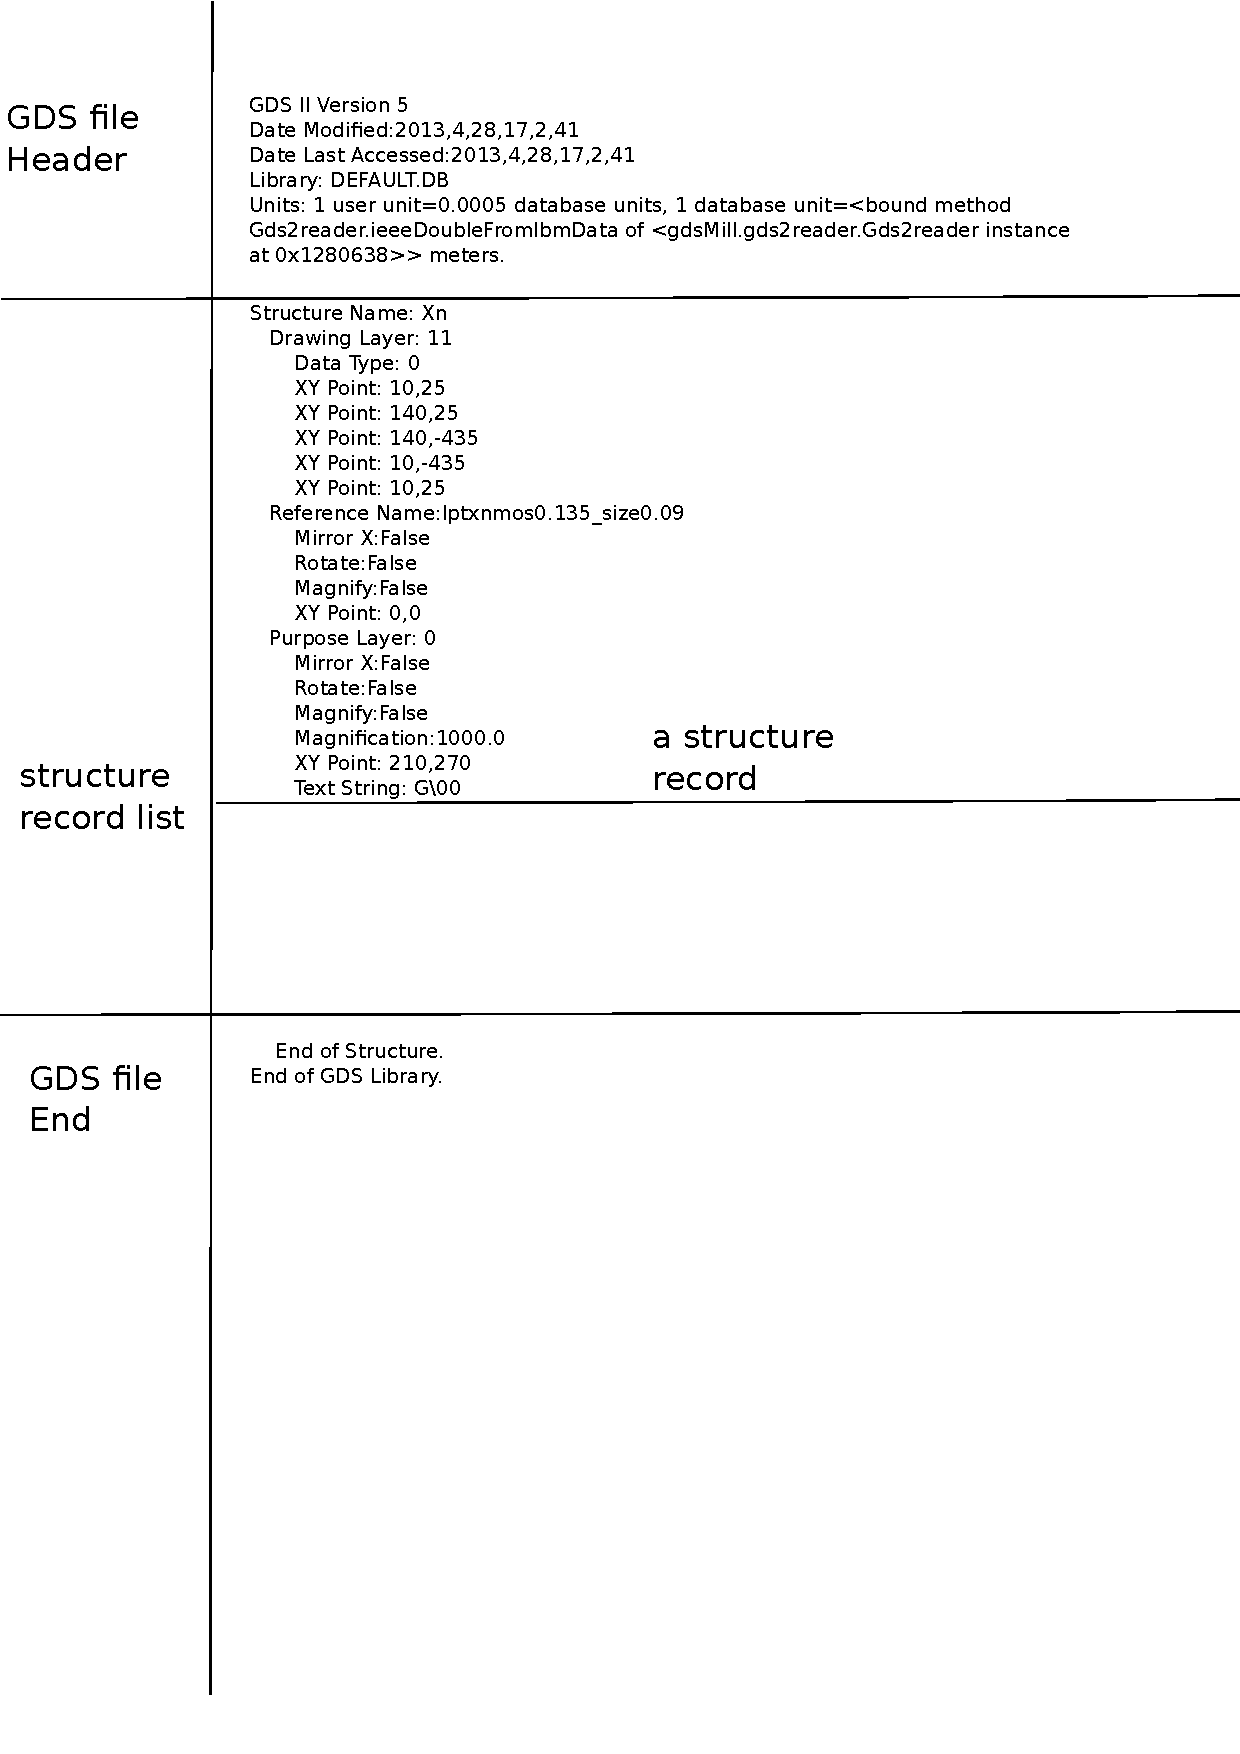
\includegraphics[width=10cm]{./figs/gds_file}
\caption{example of a GDSII file}
\label{fig:gds_file}
\end{figure}

The first part is the gds file header, which the contains GDSII
version number, date modified, date last accessed, library, user
units, and database units.

The second part is the list of structures.  These structures contain
geometries or references to other structures of the layout in
heirarchical form.  Within a structure there are several kinds of
records:

\begin{itemize}
\item Rectangle - basic geometry unit in a design, represent one layer
  of material in a circuit(i.e. a metal pin). Five coordinates and
  layer number are stored in rectangle record.
\item Structure Reference - a structure that is used in this
  structure. The information about this reference will be used store
  as a structure in the same gds file.
\item Text - a text record used for labels.
\item Path - used to represent a wire.
\item Boundary - defines a filled polygon.
\item Array Reference - specifies an array of structure instances
\item Node - Electrical nets may be specified with the NODE record
\end{itemize}

The last part is the tail of the GDSII file which ends the GDS
Library.

\fixme{Provide a link to the complete GDSII specification.}

\subsubsection{GdsMill}
\label{sec:gdsmill}

As previously stated, GdsMill is a set of scripts that can be used to read, write, and manipulate GDSII files. 

\paragraph{The gds2\_reader and gds2\_writer:}

In GdsMill, the \verb|gds2_reader| and \verb|gds2_writer| classes contain the various functions used to convert data between GDSII files and the \verb|vlsilayout| class. These classes process the data by iterating through every record in the GDS structures and check or write every data record. The record type (see Section~\ref{sec:format}),is tracked and identified using flags.

\fixme{Do we need more information of these classes, or should we just point to the GdsMill documentation?}

\paragraph{The VlsiLayout Class:}
\label{sec:vlsilayout}

After the \verb|gds2_reader| class reads in the records, the data has to be stored in a
way that can be easily used by our code. Thus, the
\verb|VlsiLayout| class is made to represent the layout.
\verb|VlsiLayout| contains the same information as GDSII file but in a
different way. \verb|VlsiLayout| stores records in data structures, which
are defined in \verb|gdsPrimitives.py|.  Each record type has a corresponding class defined in \verb|gdsPrimitives|.  Thus, a vlsilayout should at least
contains following member data:
\begin{itemize}
\item \verb|self.rootStructureName| - name of the top design.
\item \verb|self.structures| -list of structure that are used in the class. 
\item \verb|self.xyTree| - contains a list of all structure names that appeared in the design. 
\end{itemize}

The \verb|VlsiLayout| class also contains many functions for adding
structures and records to a layout class, but the important and most
useful functions have been aggregated into a wrapper file.  This
wrapper is called \verb|geometry.py| and is located in the
\verb|compiler| directory.

\subsubsection{OpenRAM-GdsMill Interface}
\label{sec:wrapper}

Dynamically generated cells and arrays each need to build a
\verb|VlsiLayout| data structure to represent the hierarchical layout.
This is performed using various functions from the \verb|VlsiLayout|
class in GdsMill, but the GdsMill file is very large and can be
difficult to understand.  To make things easier, OpenRAM has its own
wrapper class called \verb|geometry| in \verb|geometry.py|.  This
wrapper class initializes data structures for the
instances and objects that will be added to the \verb|VlsiLayout|
class.  The functions \verb|add_inst()|, \verb|add_rect()|,
\verb|add_label()| in \verb|hierarchy_layout|, add the structures to
the \verb|geometry| class, which is then written out to a GDSII file
using \verb|VlsiLayout| and the \verb|gds2_writer|.

User included library cells, which should be in gds files, can be used
as dynamically generated cells by using GDSMill.
Cell information such as cell size and pin location can be obtained by using
built in functions in the \verb|VlsiLayout| class.

Cell size can be finded by using the \verb|readLayoutBorder| function of the \verb|VlsiLayout| class.
A boundary layer should be drawn in each library cell to indicate the cell area.
The \verb|readLayoutBorder| function will return the width and height of the boundary.
If a boundary layer do not exist in the layout, then \verb|measureSize| can find the physical 
size cell.
The first method is used as primary method in \verb|auto_Measure_libcell| the lib\_utility.py,
while the second method is used as a back up one.
Each technolgy setup will import this utility function and read the library cell.

Pin location can be find by using the \verb|readPin| function of the \verb|VlsiLayout| class.
The \verb|readPin| function will return the biggest boundary which covers the label and 
is at the same layer as the label is.


\subsection{Technology Directory}
\label{sec:techdir}

The aim of creating technology directory is to make OpenRAM portable
to different technologies. This directory contains all the information
related to the specific process/technology that is being used.  In
OpenRAM, the default technology is FreePDK45, which has it own
technolony directory in the trunk.  The technology-specific directory
should consist of the following:
\begin{itemize}
\item Technology Setup FIle - In \verb|/techdir/setup_scripts|, there
  should be a Python file that sets up the PDK and defines anything
  necessary for a given technology. This file should be named
  \verb|setup_openram_<techname>.py| where techname is the name used
  to identify it in configuration scripts.
\item Technology-Specific Parameters - These parameters should include
  layer numbers and any design rules that may be needed for generating
  dynamic designs (DRC rules). The parameters should be added in
  \verb|techname/tech/tech.py| and optinally in a \verb|techname/layer.map| for
  DRC/LVS streaming. 
\item Library Cells - The library cells and corresponding spice
  netlists should be added to the \verb|techname/gds_lib| and
  \verb|techname/sp_lib| directories.
\item Spice Models - If models are not supplied in the PDK, they can be
  placed in the technology directory as done in SCMOS.
\end{itemize}

The height and width of library cells is determined by the bounding
box of all geometries. Sometimes this is not desired, for example,
when a rail must be shared. In this case, the boundary layer in the
technology file is used to define the height and width of the cell.

Pins are recognized in library cells by the largest rectangle that
encloses the pin label text. Multiple pins with the same name are
supported.  Pins with the same name such as gnd are assumed to be
``must connect'' which requires that they later be connected.

For more information regarding the technology directory and how to set
one up for a new technology, refer to Section~\ref{sec:porting}

\subsection{DRC/LVS Interface}
\label{sec:drclvs}

Each design class contains a function \verb|DRC_LVS()| that performs both
DRC and LVS on the current design module. This enables bottom-up
correct-by-construction design and easy identification of where errors
occur. It does incur some run-time overhead and can be disabled on
the command line. The \verb|DRC_LVS()| function saves a GDSII file and a Spice
file into a temporary directory and then calls two functions to
perform DRC and LVS that are tool-dependent.

Wrapper implementation for DRC and LVS functions are provided for the
open-source tools Magic+Netgen and the commercial tool, Cadence
Calibre.  Each of these functions generates a batch-mode script or runset
file which contains the options to correctly run DRC and LVS. The
functions then parse the batch mode output for any potential errors
and returns the number of errors encountered.

The function \verb|run_drc()| requires a cell name and a GDSII
file. The cell name corresponds to the top level cell in the GDSII
file. For Calibre, it also uses the layer map file for the technology
to correctly import the GDSII file into the Cadence database to
perform DRC. The function returns the number of DRC violations.

The function \verb|run_lvs()| requires a cell name, a GDSII file, and
a Spice file. Magic or Calibre will extract an extracted Spice netlist
from the GDSII file and will then compare this netlist with the
OpenRAM Spice netlist. The function returns the number of errors
encountered if there is an LVS mismatch.


For both DRC and LVS, the summary file and other report files are left
in the OpenRAM temporary directory after DRC/LVS is run. These report
files can be examined to further understand why errors were
encountered. In addition, by increasing the debug level with one or
more ``-v'' command-line parametres, the command to re-create the
DRC/LVS check can be obtained and run manually.







%%%%%%%%%%%%%%%%%%%%%%%%%%%%%%%%%%%%%%%%%%%%%%%%%%%%%%%%%%%%%%%%%%%%%%%%%%%
\section{Custom Layout Design Functions in Software}
\label{sec:parameterized}

OpenRAM provides classes that can be used to generated parameterized
cells for the most common cells: transistors, inverters, nand2, nand3, etc...  
There are many advantages to having parameterized cells.
The main advantage is that it makes it easier to dynamically generate designs and cuts
down the necessary code to be written.  
We also need parameterized cells because some designs, such as the wordline drivers, need to be
dynamically sized based on the size of the memory. 
Lastly, there may be certain physical dimension requirements that need to be met for a
cell, while still maintaing the expected operation/performance.  
In OpenRAM we currently provide five parameterized cells: parameterized
transistor (\verb|ptx|), parameterized inverter (\verb|pinv|), parameterized nand2 (\verb|nand_2|), 
parameterized nand3 (\verb|nand_3|) and parameterized nor2 (\verb|nor_2|). 


\subsection{Parameterized Transistor}
\label{sec:ptx}

The parameterized transistor class generates a transistor of specified
width and number of mults.
The \verb|ptx| is constructed as follows:
\begin{verbatim}
def __init__(self,name,width,mults,tx_type)
\end{verbatim} 

An explanation of the \verb|ptx| parameters is shown in
Table~\ref{table:ptx_params}. A layout of ptx, generated by the
following instatiation, is depicted in Figure~\ref{fig:ptx_example}.
\begin{verbatim}
fet = ptx.ptx(name = "nmos_1_finger", width = tech.drc["minwidth_tx"], 
mults = 1, tx_type = "nmos").
\end{verbatim}

\begin{table}[h!] 
  \begin{center}
    \begin{tabular}{| l | c |}
    \hline
    Parameter & Explanation  \\ \hline
    \verb|width| & active\_height \\ \hline
    \verb|mults| & mult number of the transistor \\ \hline
    \verb|tx_type| & type of transistor,”nmos” and “pmos” \\ \hline
    \hline
    \end{tabular}
  \end{center}
  \caption{Parameter Explanation of ptx}
  \label{table:ptx_params}
\end{table}


\begin{figure}[h!]
\centering
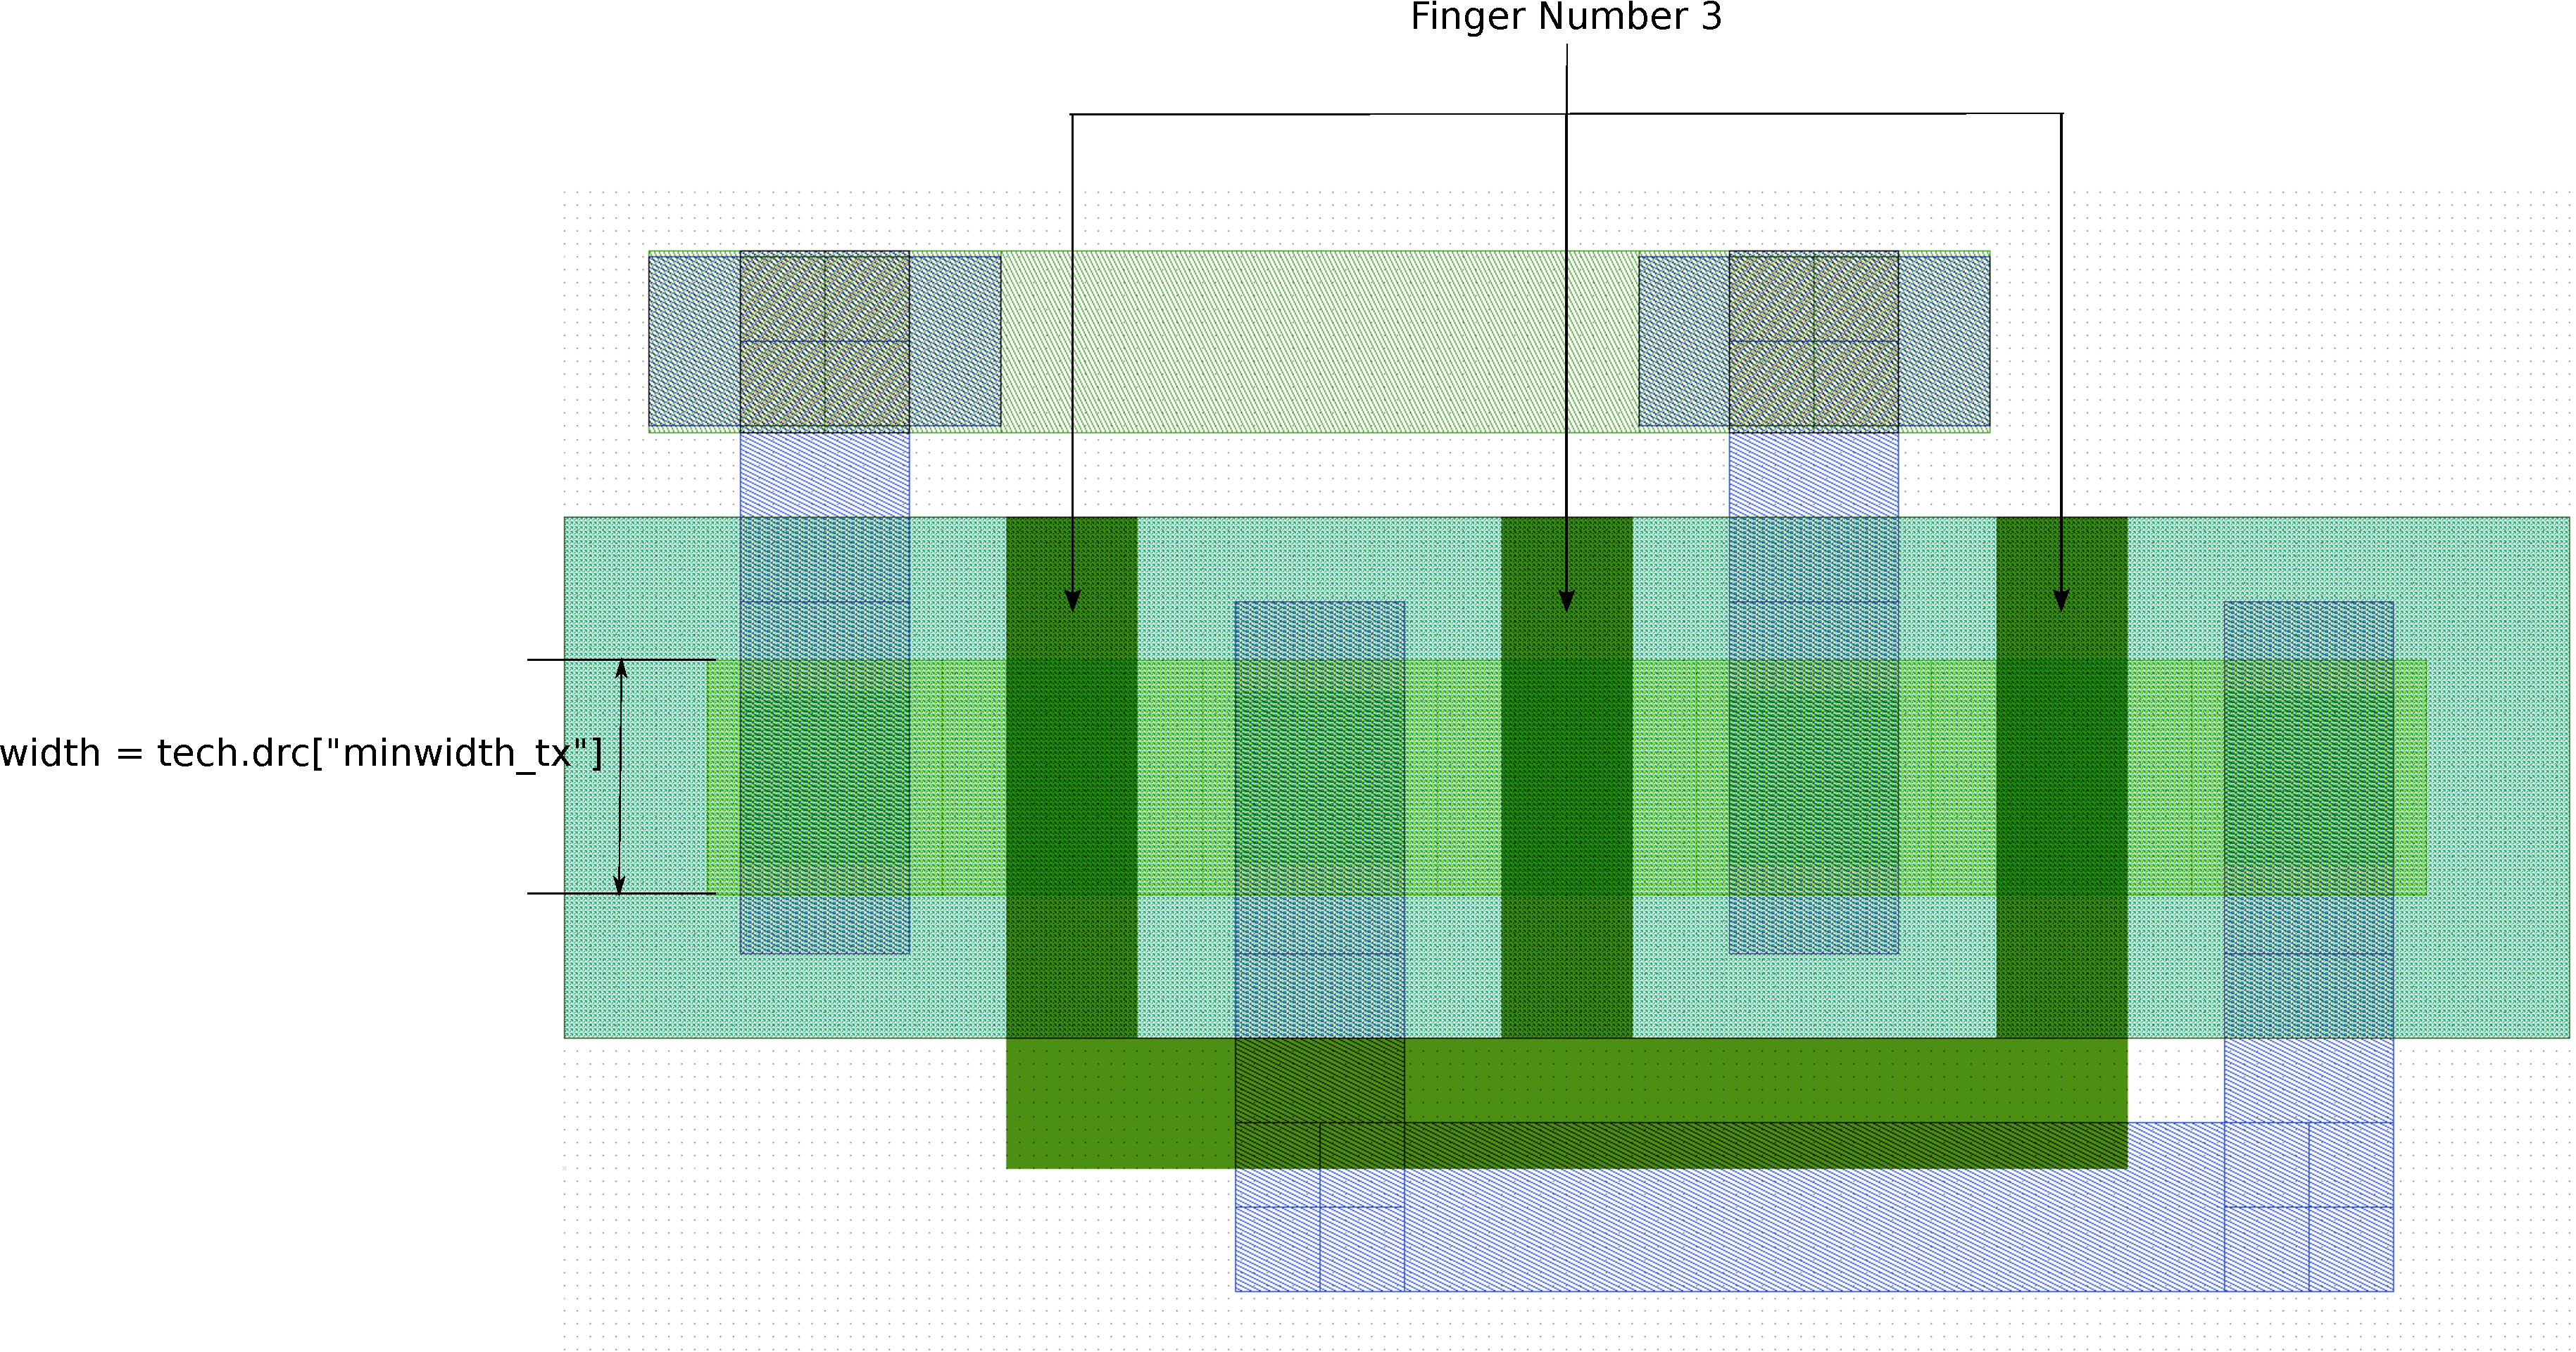
\includegraphics[width=10cm]{./figs/ptx.pdf}
\caption{An example of Parameterized Transistor (ptx)}
\label{fig:ptx_example}
\end{figure}



\subsection{Parameterized Inverter}
\label{sec:pinv}

The parameterized inverter (\verb|pinv|) class generated an inverter
of a specified size/strength and height.  The \verb|pinv| is
constructed as follows:
\begin{verbatim}
def __init__(self, cell_name, size, beta=tech.[pinv.beta], 
cell_size=tech.cell[height])
\end{verbatim}

The parameterized inverter can provide significant drive strength
while adhering to physical cell size limitations. That is achieved by
having many small transistors connected in parallel, thus the height
of the inverter cell can be manipulated without the affecting the
drive strength. The NMOS size is an input parameter, and the PMOS size
will be determined by $beta*NMOS\_size$, where beta is the ratio of
the PMOS channel width to the NMOS channel width.  The following code
instatiates the \verb|pinv| instance seen in Figure~\ref{fig:pinv}.
\begin{verbatim}
a=pinv.pinv(cell_name="pinv",size=tech.drc["minwidth_tx"]*8)
\end{verbatim}
\begin{figure}[h!]
\centering
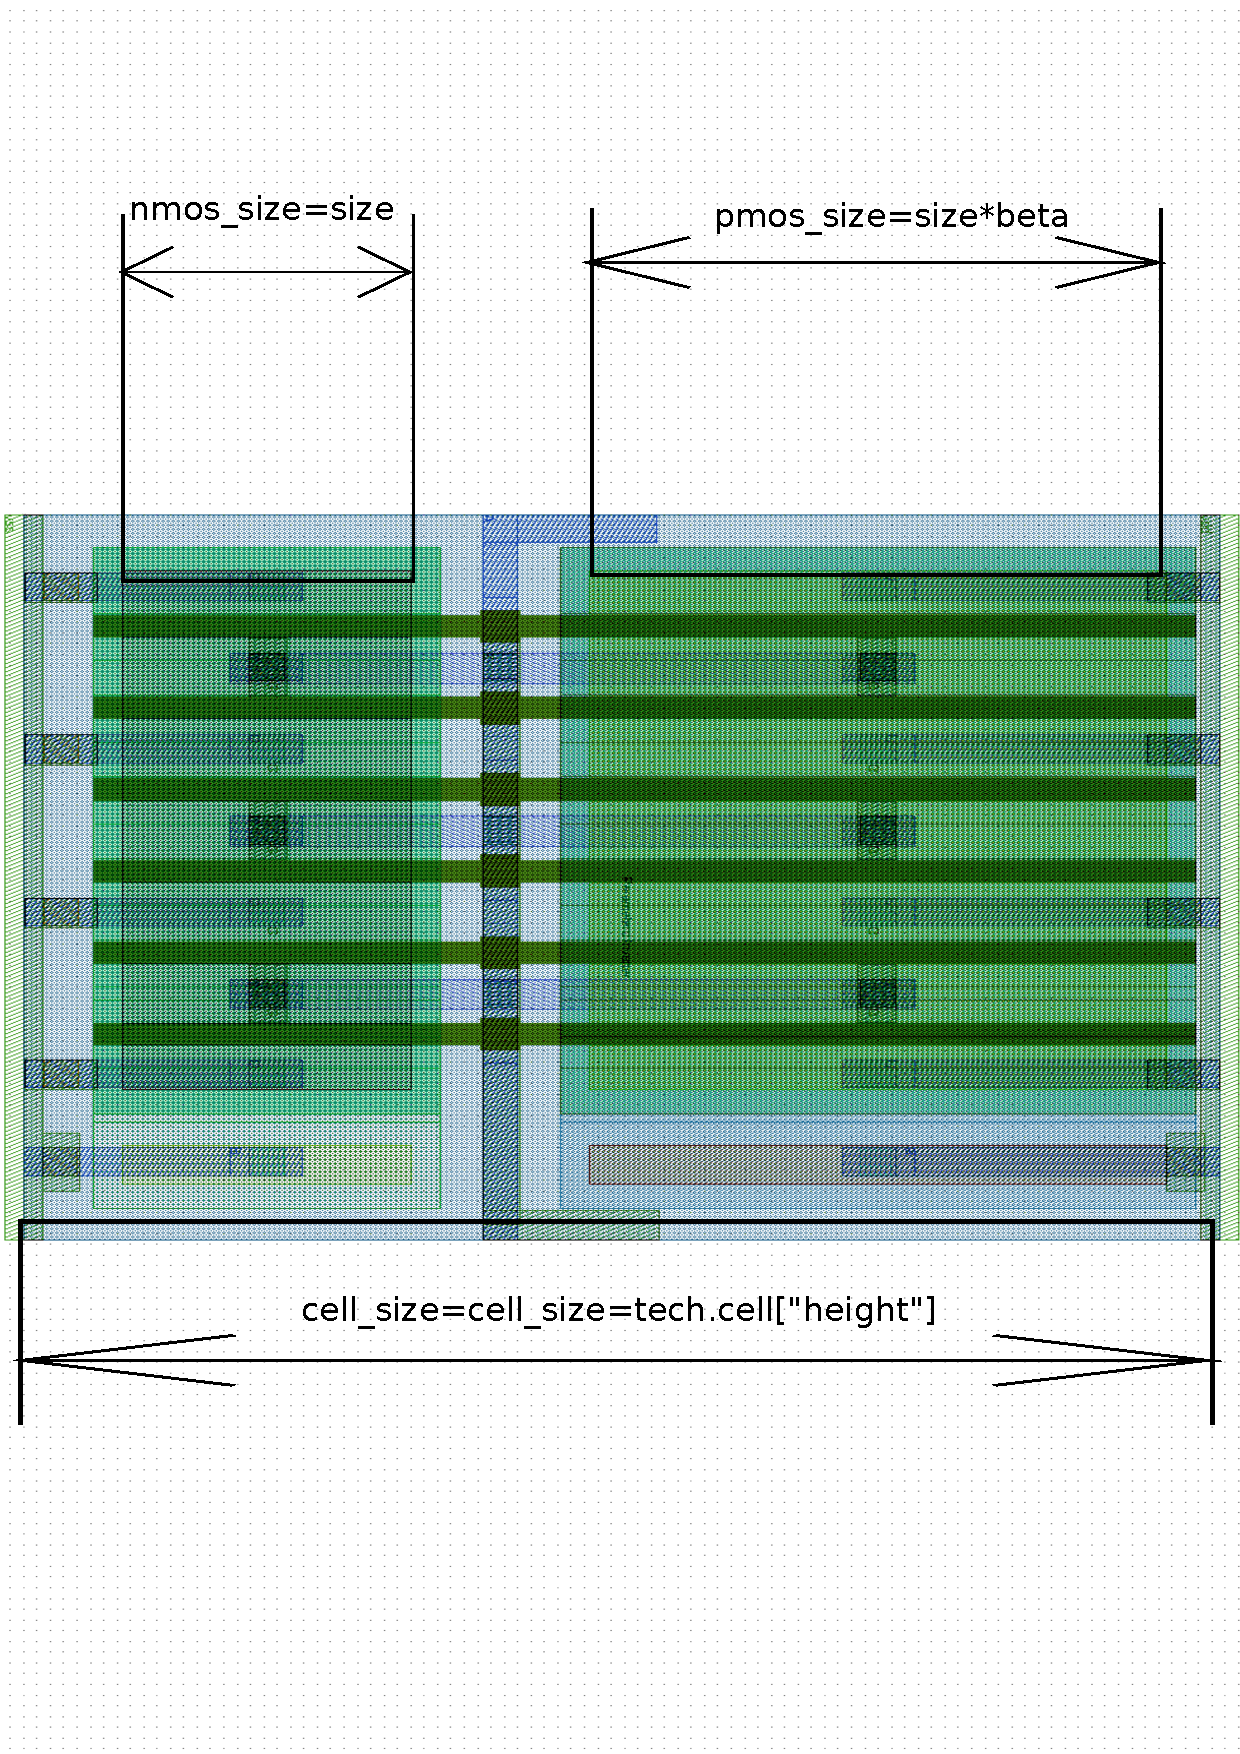
\includegraphics[width=10cm]{./figs/pinv.pdf}
\caption{An example of Parameterized Inverter(pinv)}
\label{fig:pinv}
\end{figure}


The \verb|pinv| parameters are explained in Table~\ref{table:pinv_params}.
\begin{table}[h!] 
  \begin{center}
    \begin{tabular}{| l | c |}
    \hline
    Parameter & Explanation \\ \hline
    \verb|size| & The logic size of the transistor of the nmos in the pinv \\ \hline
    \verb|beta| = tech.[pinv.beta] & Ratio of pmos channel width to nmos channel width. \\ \hline
    \verb|cell_size| = tech.cell[height] & physical dimension of cell height. \\ 
    \hline
    \end{tabular}
  \end{center}
  \caption{Parameter Explanation of pinv}
  \label{table:pinv_params}
\end{table}



\subsection{Parameterized NAND2}
\label{sec:nand2}

The parameterized nand2 (\verb|nand_2|) class generated a 2-input nand gate
of a specified size/strength and height.  The \verb|nand_2| is
constructed as follows:
\begin{verbatim}
def __init__(self, name, nmos_width, height=tech.cell_6t[height])
\end{verbatim}

The NMOS size is an input parameter, and the PMOS size
will be equal to NMOS to have the equal rising and falling for output. 
The following code instatiates the \verb|nand_2| instance seen in Figure~\ref{fig:nand2}.
\begin{verbatim}
a=nand_2.nand_2(name="nand2", nmos_width=2*tech.drc["minwidth_tx"], 
height=tech.cell_6t["height"])
\end{verbatim}

\begin{figure}[h!]
\centering
%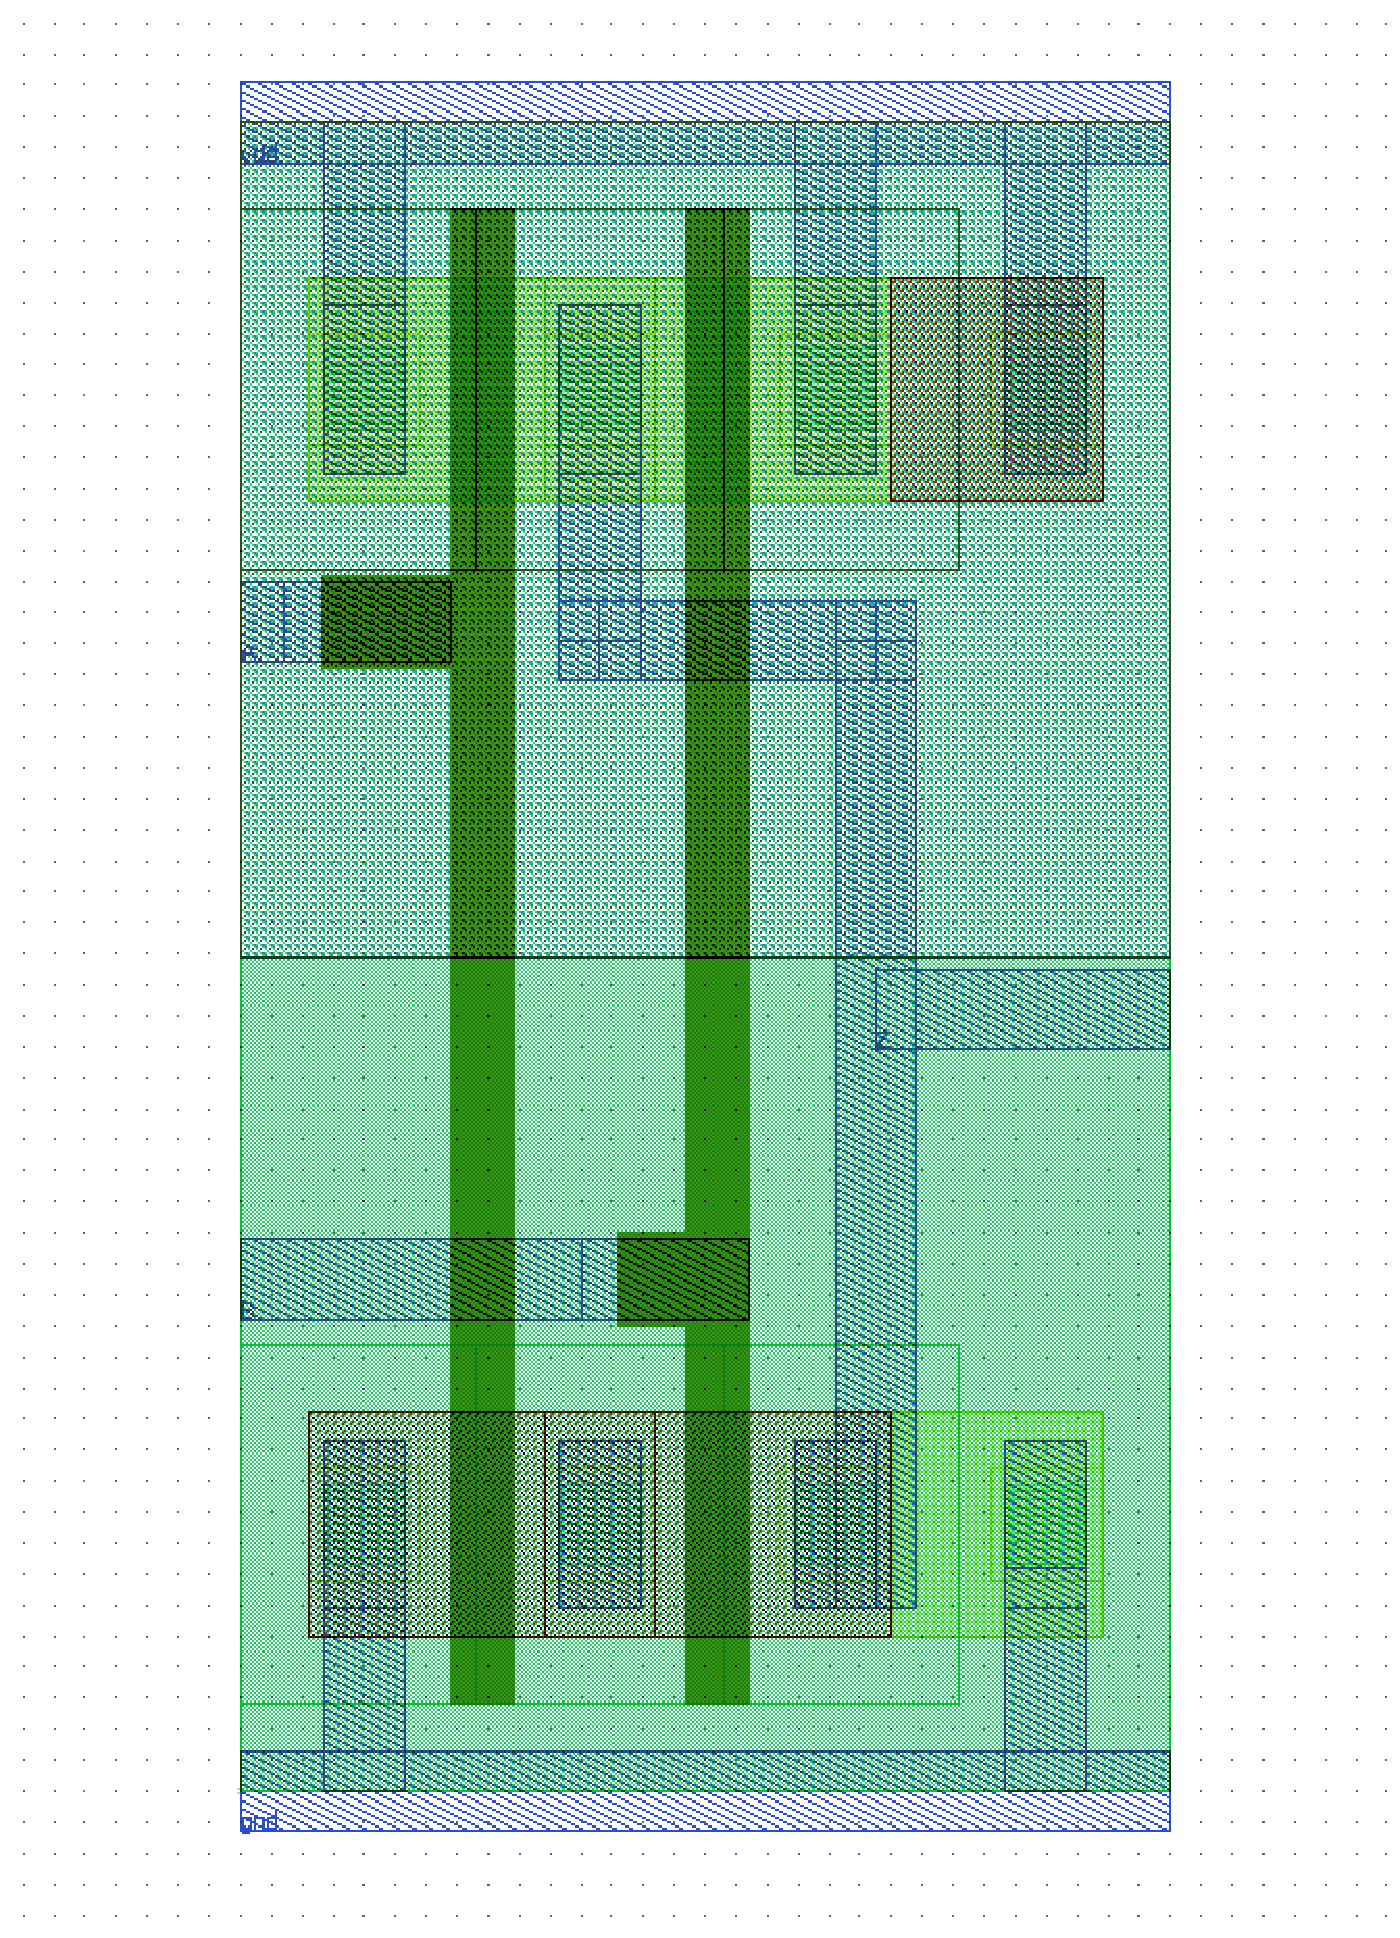
\includegraphics[width=10cm]{./figs/nand2.pdf}
\caption{An example of Parameterized NAND2(nand\_2)}
\label{fig:nand2}
\end{figure}


The \verb|nand_2| parameters are explained in Table~\ref{table:nand2_params}.
\begin{table}[h!] 
  \begin{center}
    \begin{tabular}{| l | c |}
    \hline
    Parameter & Explanation \\ \hline
    \verb|nmos_width| & The logic size of the transistor of the nmos in the nand2 \\ \hline
    \verb|height| = tech.cell\_6t[height] & physical dimension of cell height. \\ 
    \hline
    \end{tabular}
  \end{center}
  \caption{Parameter Explanation of nand2}
  \label{table:nand2_params}
\end{table}



\subsection{Parameterized NAND3}
\label{sec:nand3}

The parameterized nand3 (\verb|nand_3|) class generated a 3-input nand gate
of a specified size/strength and height.  The \verb|nand_3| is
constructed as follows:
\begin{verbatim}
def __init__(self, name, nmos_width, height=tech.cell_6t[height])
\end{verbatim}
The NMOS size is an input parameter, and the PMOS size
will be equal to $2/3$ NMOS size to have the equal rising and falling for output.
The following code instatiates the \verb|nand_3| instance seen in Figure~\ref{fig:nand3}.
\begin{verbatim}
a=nand_3.nand_3(name="nand3", nmos_width=3*tech.drc["minwidth_tx"], 
height=tech.cell_6t["height"])
\end{verbatim}


\begin{figure}[h!]
\centering
%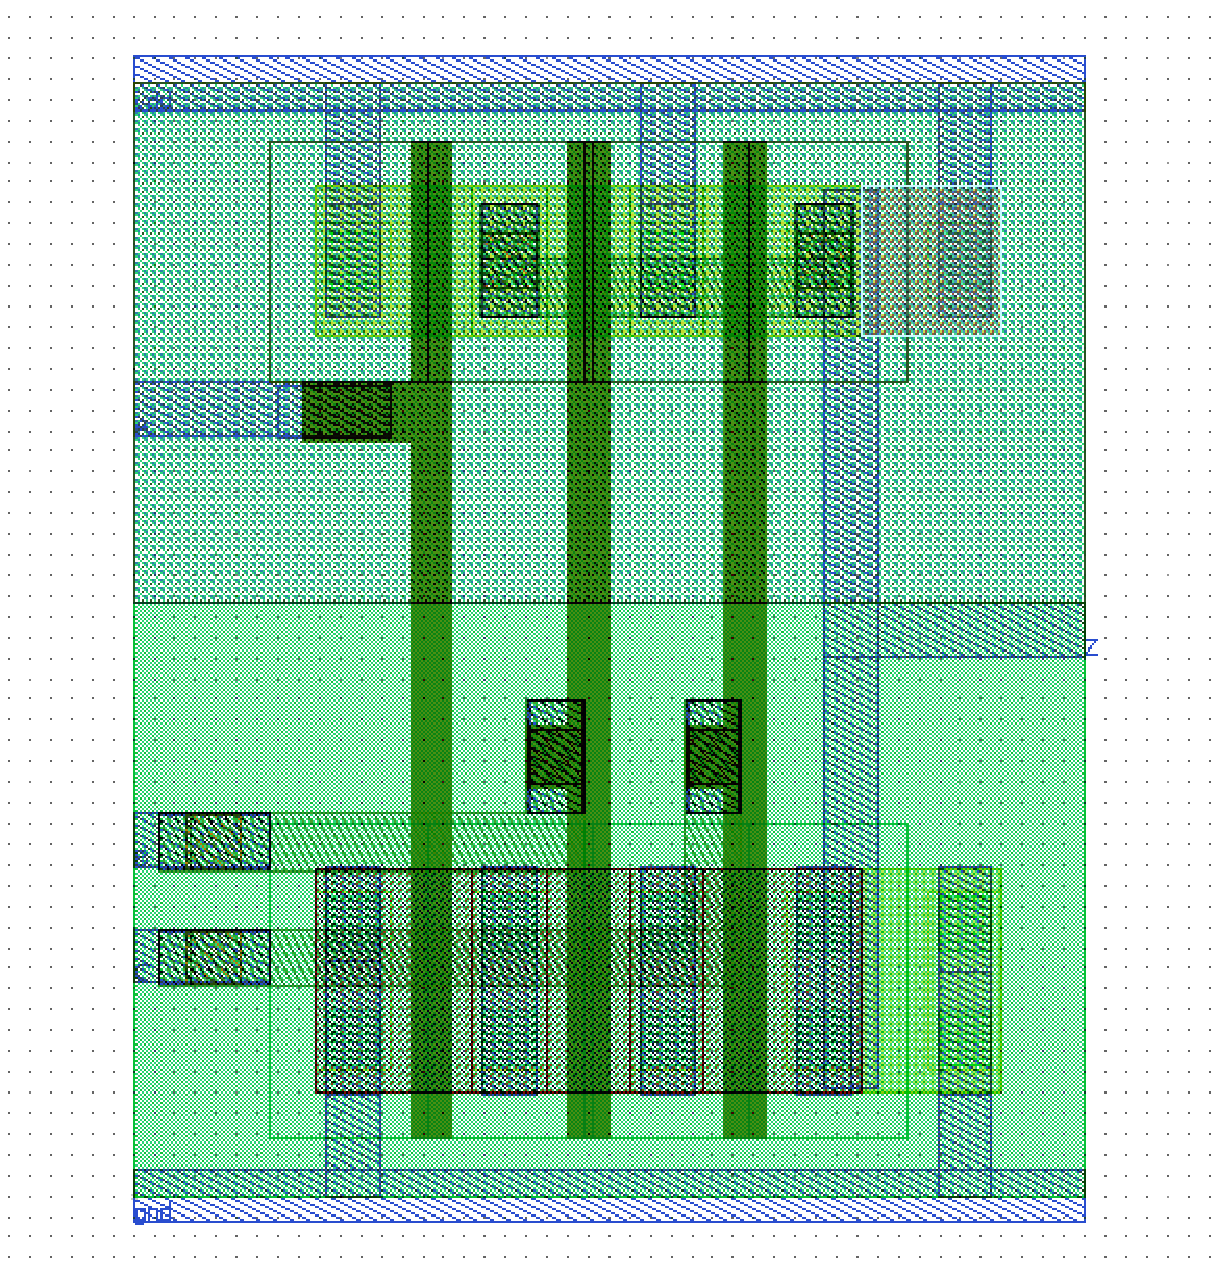
\includegraphics[width=10cm]{./figs/nand3.pdf}
\caption{An example of Parameterized NAND3(nand\_3)}
\label{fig:nand3}
\end{figure}

The \verb|nand_3| parameters are explained in Table~\ref{table:nand3_params}.
\begin{table}[h!] 
  \begin{center}
    \begin{tabular}{| l | c |}
    \hline
    Parameter & Explanation \\ \hline
    \verb|nmos_width| & The logic size of the transistor of the nmos in the nand3 \\ \hline
    \verb|height| = tech.cell\_6t[height] & physical dimension of cell height. \\ 
    \hline
    \end{tabular}
  \end{center}
  \caption{Parameter Explanation of nand3}
  \label{table:nand3_params}
\end{table}


\subsection{Parameterized NOR2}
\label{sec:nor2}

The parameterized nor2 (\verb|nor_2|) class generated a 2-input nor gate
of a specified size/strength and height.  The \verb|nor_2| is
constructed as follows:
\begin{verbatim}
def __init__(self, name, nmos_width, height=tech.cell_6t[height])
\end{verbatim}
The NMOS size is an input parameter, and the PMOS size
will be equal to $2$ NMOS size to have the equal rising and falling for output.
The following code instatiates the \verb|nor_2| instance seen in Figure~\ref{fig:nor2}.
\begin{verbatim}
a=nor_2.nor_2(name="nor2", nmos_width=2*tech.drc["minwidth_tx"], 
height=tech.cell_6t["height"])
\end{verbatim}


\begin{figure}[h!]
\centering
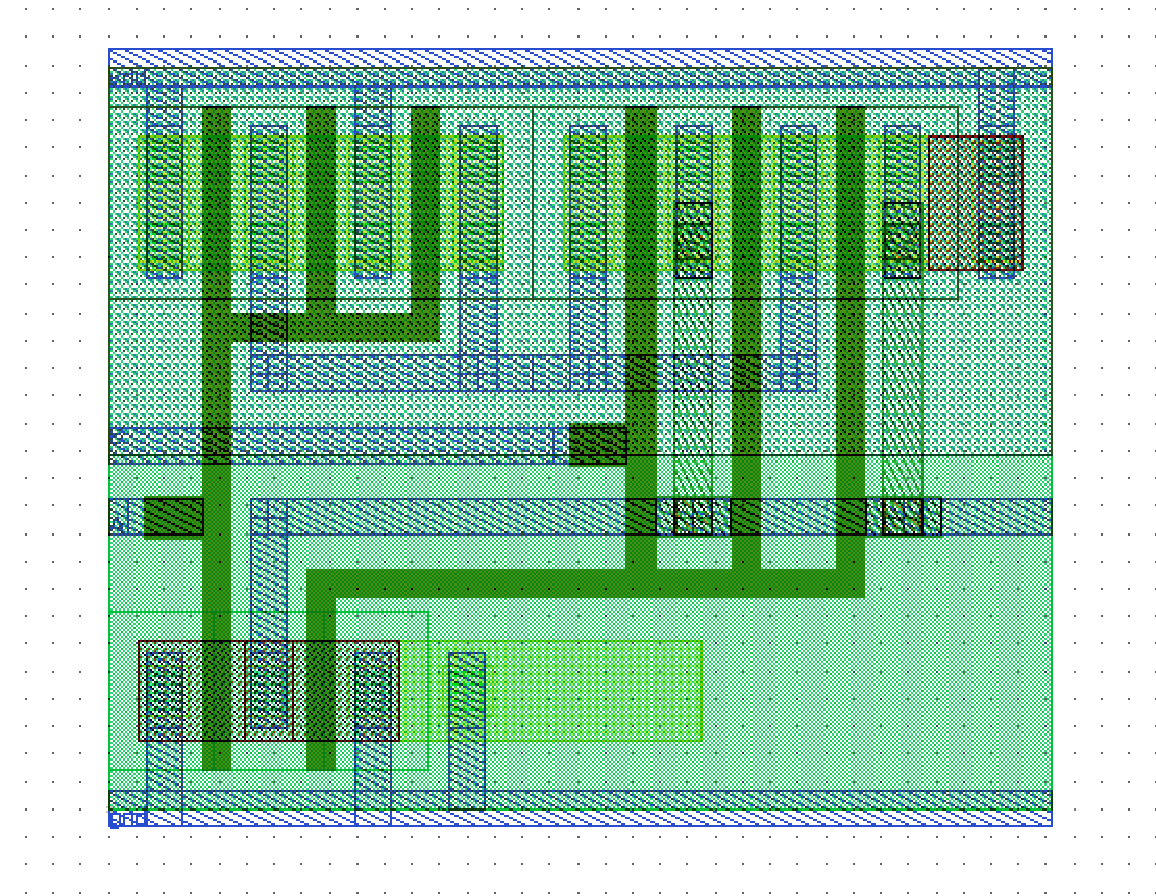
\includegraphics[width=10cm]{./figs/nor2.pdf}
\caption{An example of Parameterized NOR2(nor\_2)}
\label{fig:nor2}
\end{figure}

The \verb|nor_2| parameters are explained in Table~\ref{table:nor2_params}.
\begin{table}[h!] 
  \begin{center}
    \begin{tabular}{| l | c |}
    \hline
    Parameter & Explanation \\ \hline
    \verb|nmos_width| & The logic size of the transistor of the nmos in the nor2 \\ \hline
    \verb|height| = tech.cell\_6t[height] & physical dimension of cell height. \\ 
    \hline
    \end{tabular}
  \end{center}
  \caption{Parameter Explanation of nor2}
  \label{table:nor2_params}
\end{table}



\subsection{Path and Wire}
\label{sec:path and wire}
OpenRam provides two routing classes in custom layout design.
Both Path and wire class will take a set of coordinates connect those points 
with rectilinear metal connection.

The difference is that path only use the same layers for both vertical and 
horizontal connection while wire will use two different adjacent metal layers.
The this example will construct a metal1 layer path
\begin{verbatim}
layer_stack = ("metal1")
position_list = [(0,0), (0,3), (1,3), (1,1), (4,3)]
w=path.path(layer_stack,position_list) 
\end{verbatim}
and This exmaple will construct a wire using metal1 for vertical connection and metal2 for 
horizontal connection:
\begin{verbatim}
layer_stack = ("metal1","via1","metal2")
position_list = [(0,0), (0,3), (1,3), (1,1), (4,3)]
w=wire.wire(layer_stack,position_list)
\end{verbatim}





%%%%%%%%%%%%%%%%%%%%%%%%%%%%%%%%%%%%%%%%%%%%%%%%%%%%%%%%%%%%%%%%%%%%%%%%%%%
\section{Porting to a new Technologies}
\label{sec:porting}

The folllowing sub-directories and files should be added to your new technology directory:
\begin{itemize}
\item \verb|/sp_lib| - spice netlists for library cells
\item \verb|/gds_lib| - GDSII files for the library cell
\item \verb|layers.map| - layer/purpose pair map from the technology
\item \verb|/tech| - contains tech parameters, layers, and portation functions.
\end{itemize}

\subsection{The GDS and Spice Libraries}

The GDS and Spice libraries , \verb|\gds_lib| and \verb|\sp_lib|, should contain the GDSII layouts and spice netlists for each of the library cells in your SRAM design.  For the FreePDK45 technology, library cells for the 6T Cell, Sense Amp, Write Driver, Flip-Flops, and Control Logic are provided.  To reiterate: all layouts must be exported in the GDSII file format.  The following commands can be used to stream GDSII files into or out of Cadence Virtuoso:
\begin{verbatim}
To stream out of Cadence:

  strmout -layerMap ../sram_lib/layers.map 
    -library sram -topCell $i -view layout 
      -strmFile ../sram_lib/$i.gds

To stream a layout back into Cadence:

  strmin -layerMap ../sram_lib/layers.map 
    -attachTechFileOfLib NCSU_TechLib_FreePDK45 
       -library sram_4_32 -strmFile sram_4_32.gds
\end{verbatim}
When you import a gds file, make sure to attach the correct tech lib or you will get incorrect layers in the resulting library.



\subsection{Technology Directory}
\label{sec:tech}

Inside of the \verb|/tech| directory should be the Python classes for \verb|tech.py|,
\verb|ptx_port.py|, and any other portation functions.  The \verb|tech.py| file is very important and should contain the following:
\begin{itemize}
\item Layer Number/Name - GDSII files only contain layer numbers and it can be difficult to keep track of which layer corresponds to what number.  In OpenRAM code, layers are referred to by name and \verb|tech.py| maps the layer names that we use to the layer numbers in the \verb|layer.map|  This will associate the layer name used in OpenRAM program with the number used in the layer.map, thus the code in complier won’t need to be changed for each technology.
\item Tech Parameters - important rules from the DRC rule deck(such as layer spacing and minimum sizes) should be included here.  Please refer to the rules that are included in \verb|tech.py| to get a better idea as to what is important.
\item Cell Sizes and Pin Offsets - The \verb|cell_size()| and \verb|pin_finder()| functions should be used to populate this class with the various cell sizes and pin locations in your library cells.  These functions are relatively slow because they must traverse the every shape in the entire hierarchy of a design.  Due to this fact, these function are not invoked each time the compiler is run, it should be run one time or if any changes have been made to library cells. This sizes and pin locations gathered are needed to generate the dynamic cells and perform routing at the various levels of the hierarchy.  It is suggested that boundary boxes on a specific layer should be added to define the cell size.
\end{itemize}








%%%%%%%%%%%%%%%%%%%%%%%%%%%%%%%%%%%%%%%%%%%%%%%%%%%%%%%%%%%%%%%%%%%%%%%%%%%
\section{Timing and Control Logic}
\label{timing}

This section outlines the necessary signals, timing considerations, and control circuitry for a synchronous SRAM.

\subsection{Signals}
\label{signals}
Top-Level Signals:
\begin{itemize}
\setlength{\itemsep}{0pt}
\item ADDR - address bus.
\item DATA - bi-directional data bus.
\item clk - the global clock.
\item OEb - active low output enable.
\item CSb - active low chip select.
\item WEb - active low write enable.
\end{itemize}

Internal Signals:
\begin{itemize}
\setlength{\itemsep}{0pt}
\item clk\_bar - enables the precharge unit.
\item s\_en - enables the sense amp during a read operation.
\item w\_en - enable the write driver during a write operation.
\item tri\_en and tri\_en\_bar - enable the data input tri-gate during a read operation.
\end{itemize}

\subsection{Timing Considerations}
\label{timing_params}

The main timing considerations for an SRAM are:
\begin{itemize}
\setlength{\itemsep}{0pt}
\item Setup Time - time an input needs to be stable before the positive/negative clock edge.
\item Hold Time - time an input needs to stay valid after the positive/negative clock edge.  
\item Minimun Cycle Time - time inbetween subsequent memory operations.
\item Memory Read Time - time from negative clock edge until valid data appears on the data bus.
\item Memory Write Time - time from negative clock edge until data has been driven into a memory cell.
\end{itemize}

\subsection{SRAM Operation}
\label{operation}

\begin{figure}[tb]
\centering
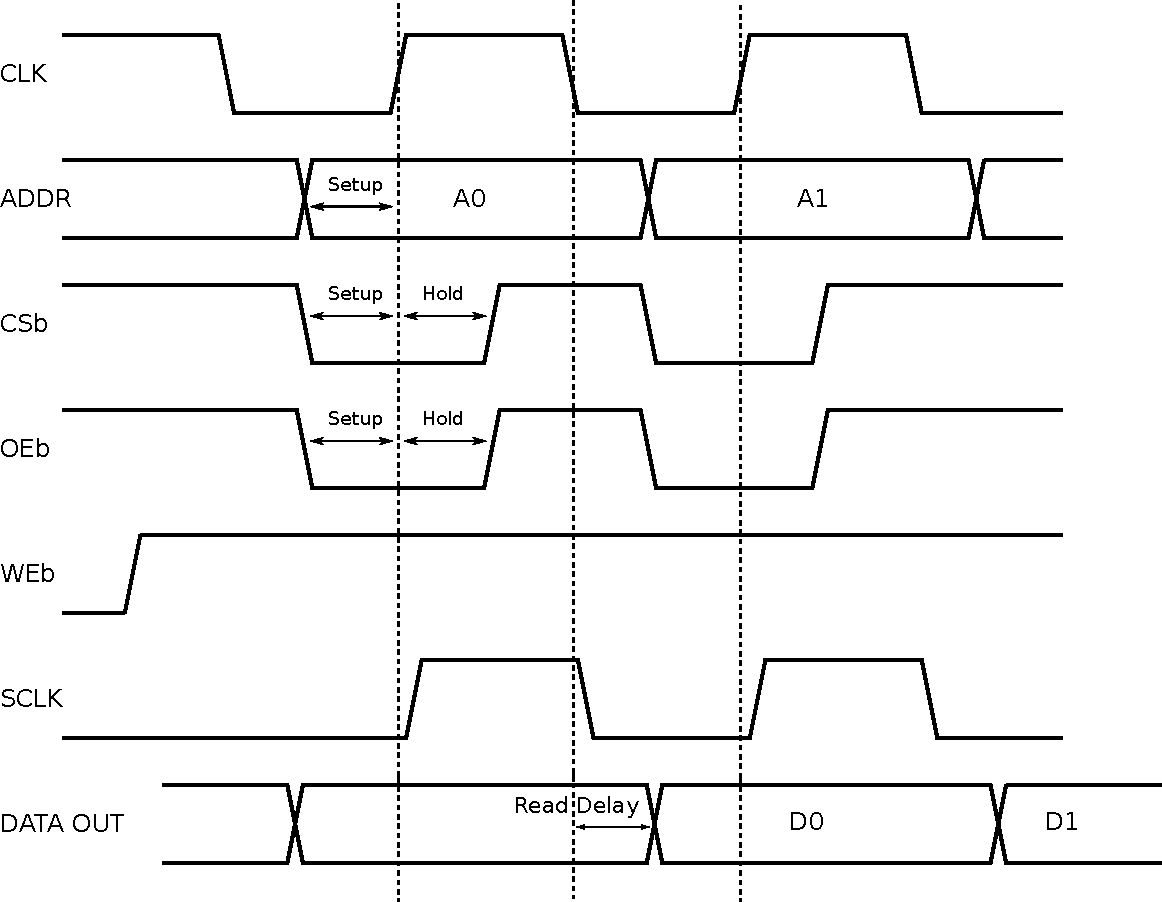
\includegraphics[scale=.85]{./figs/timing_read.pdf}
\caption{Timing diagram for read operation showing the setup, hold, and read times.}
\label{fig:read}
\end{figure}

Read Operation:
\begin{enumerate}
\setlength{\itemsep}{0pt}
 \item Before the clock transition (low to high) that initiates the read operation:
  \begin{enumerate}
	\item The chip must be selected (CSb low).
	\item The WEb must be high (read). 
	\item The row and column addresses must be applied to the address input pins (ADDR).
	\item OEb should be selected (OEb low).
   \end{enumerate}
 \item On the rising edge of the clock (CLK):
   \begin{enumerate}
	\item The control signals and address are latched into flip-flops and the read cycle begins. 
	\item The precharging of the bit lines starts.  
	\item The address bits become available for the decoder and column mux, which select the row and columns that we want to read from.
   \end{enumerate}
 \item On the falling edge of the clock (CLK):
   \begin{enumerate}
        \item Word line is driven onto the bitlines, the value stored in the memory cells pulls down one of the bitlines (bl if a 0 is stored, br if a 1 is stored).
	\item s\_en enables the sense amplifier which senses the voltage difference of the bit lines, produces the output and keeps the value in its latch circuitry.
	\item Tri-gate drives (tri\_en and tri\_en\_bar) the output data on data bus. Data remains valid on the data bus for a complete clock cycle.
   \end{enumerate}
\end{enumerate}


\begin{figure}[tb]
\centering
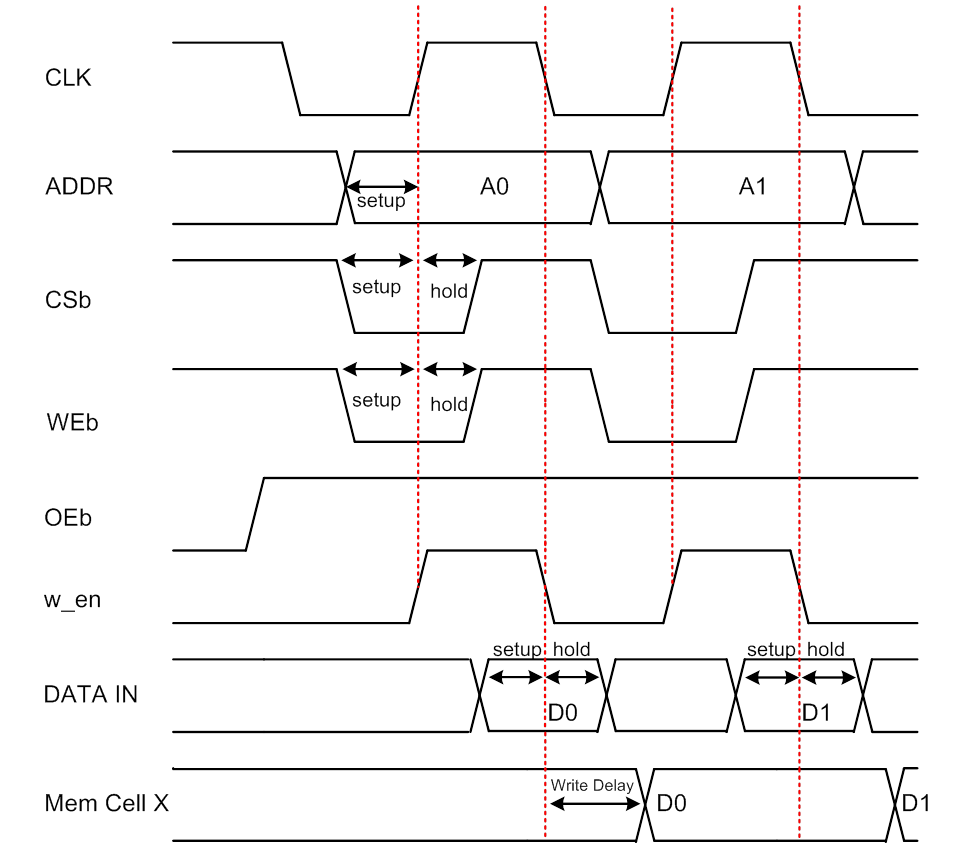
\includegraphics[scale=.9]{./figs/timing_write.pdf}
\caption{Timing diagram for write operation showing the setup, hold, and write times.}
\label{fig:write}
\end{figure}



Write Operation:
\begin{enumerate}
\setlength{\itemsep}{0pt}
 \item Before the clock transition (low to high) that initiates the write operation:
  \begin{enumerate}
	\item The chip must be selected (CSb low).
	\item The WEb must be low to enable the data input tristates.
	\item The row and column addresses must be applied to the address input pins (ADDR).
	\item OEb must be high (no output is available and sense amp disabled)
  \end{enumerate}
 \item On the rising edge of the clock (CLK):
   \begin{enumerate}
	\item OEb stays high (no output is available and sense amp disabled)
	\item The inputs addresses are latched into flip-flops, precharging starts, and the write operation begins.
	\item The address bits become available for the decoder and column mux, which select the row and columns that we want to write to.
  \end{enumerate}	         
 \item On the falling edge of the clock (CLK):
   \begin{enumerate}
	\item The data to be written must be applied to DATA and latched into flip-flops.
	\item w\_en enables the write driver, which drives the data input through the column mux and into the selected memory cells.  The write delay is the time from the negative clock edge until the data value is stored in the memory cell on node X.
   \end{enumerate}
\end{enumerate}


\subsection{Zero Bus Turnaround (ZBT)}
\label{sec:ZBT}

In timing of SRAM, during a read operation, data should be available after the clock edge while 
during a write, data should be set up before the clock edge. Due to this issue a wait state (dead cycle) is neccessary when SRAM switches 
from read mode to write mode. 
To avoide dead cycles in SRAM timing which slow down the operation and degrade the performance of SRAM, Zero Bus turnaround (ZBT) technique is used.
Using ZBT, during a write, data is set up after positive clock edge and before negative clock edge and input data is latched in negative edge flip-flops. 
Using ZBT, we will get a higher memory throughput and there is no waite states.
Figure~\ref{fig:write} shows the correct timing for input signals during the write opertion to avoide the wait states. 
Figure~\ref{fig:ZBT} shows how a write cycle is followed by a read cycle with no wait state through using ZBT.
Input address bits should be ready before positive edge to be loaded to positive edge flip-flops. Output data is ready to be loaded to data-bus during seconde half of cycle (after negative edge of clock) and 
input data should be ready before negative edge of clock to be loaded in negative edge  flip-flops.

\begin{figure}[h!]
\centering
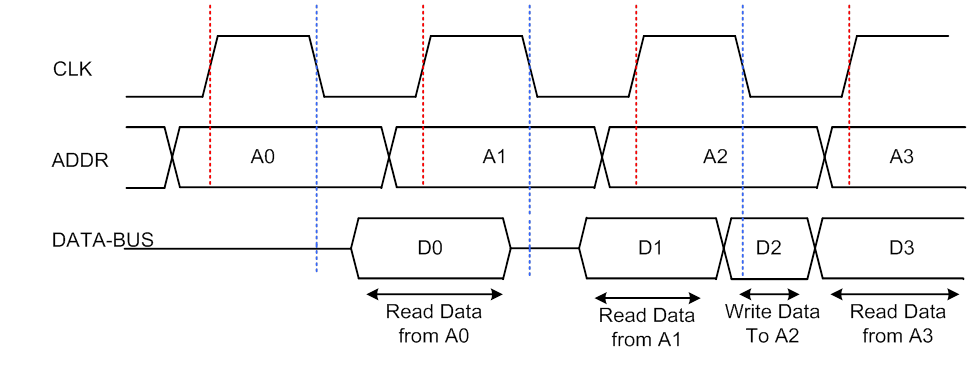
\includegraphics[scale=0.9]{./figs/ZBT.pdf}
\caption{(a) Zero Bus Turnaround timing.}
\label{fig:ZBT}
\end{figure}


\subsection{Control Logic}
\label{sec:control}



The control circuitry ensures that the SRAM operates as intended during a read or write cycle by enabling the necessary structures in the SRAM. 
As shown in Figure~\ref{fig:control}, the control logic takes three active low signals as inputs: chip select bar ($CSb$), 
output enable bar ($OEb$), and write enable bar ($WEb$). $CSb$ enables the entire SRAM chip. 
When $CSb$ is low, the appropriate control signals are generated and sent to the architecture blocks.  
Conversely, if $CSb$ is high then no control signals are generated and SRAM is turned off or disabled. 
The $OEb$ signal signifies a read operation; while it is low the value seen on the data bus will be an output from the memory. 
Similarly, the $WEb$ signal signifies a write operation. All of the input control signals are latched with master-slave flip-flops, 
ensuring that the control signal stays valid for the entire operation cycle. The control signal flip-flops use the normal clock to generate 
local signals used to enable or disable structures based on the operation. Address flip-flops are combined with global clock as well. 
In a standard write SRAM, switching from a read to a write operation results in a dead cycle. To avoid this dead cycle, Data flip-flops are 
latched with $clk\_bar$ in order to have a Zero Bus Turnaround (ZBT) memory. More details on ZBT timing are outlined in Section~\ref{sec:ZBT}. 
After all control signals are latched, they are ANDED with the $clk\_bar$ because the read/write circuitries should only be enabled after the precharging of 
the bitlines had ended on the negative edge of the clock. The $w\_en$ signal enables the write driver during a write to the memory .The $s\_en$ signal 
is generated using a Replica Bitline ($RBL$) to enable the sense amplifier during a read operation. Details on $RBL$ architecture are outlined in section~\ref{sec:RBL}. 
$tri\_en$ and $tri\_en\_bar$ enable the tristates during read in order to drive the outputs onto the data bus. 
Table~\ref{table:control} shows the truth table for the control logic. The $s\_en$ signal to enable the sense amplifier is 
true when $(CS  .  OE  .  Clk\_bar)$ is true. Similarly, write driver enable signal, $w\_en$, is true when $(CS  .  WE .  clk\_bar)$ is true.  
$tri\_en$ and $tri\_en\_bar$ are true when $\neg(OEb\_bar  |  clk)$ and $\neg(OEb  .  clk\_bar)$ are true, respectively.
\begin{figure}[h!]
\centering
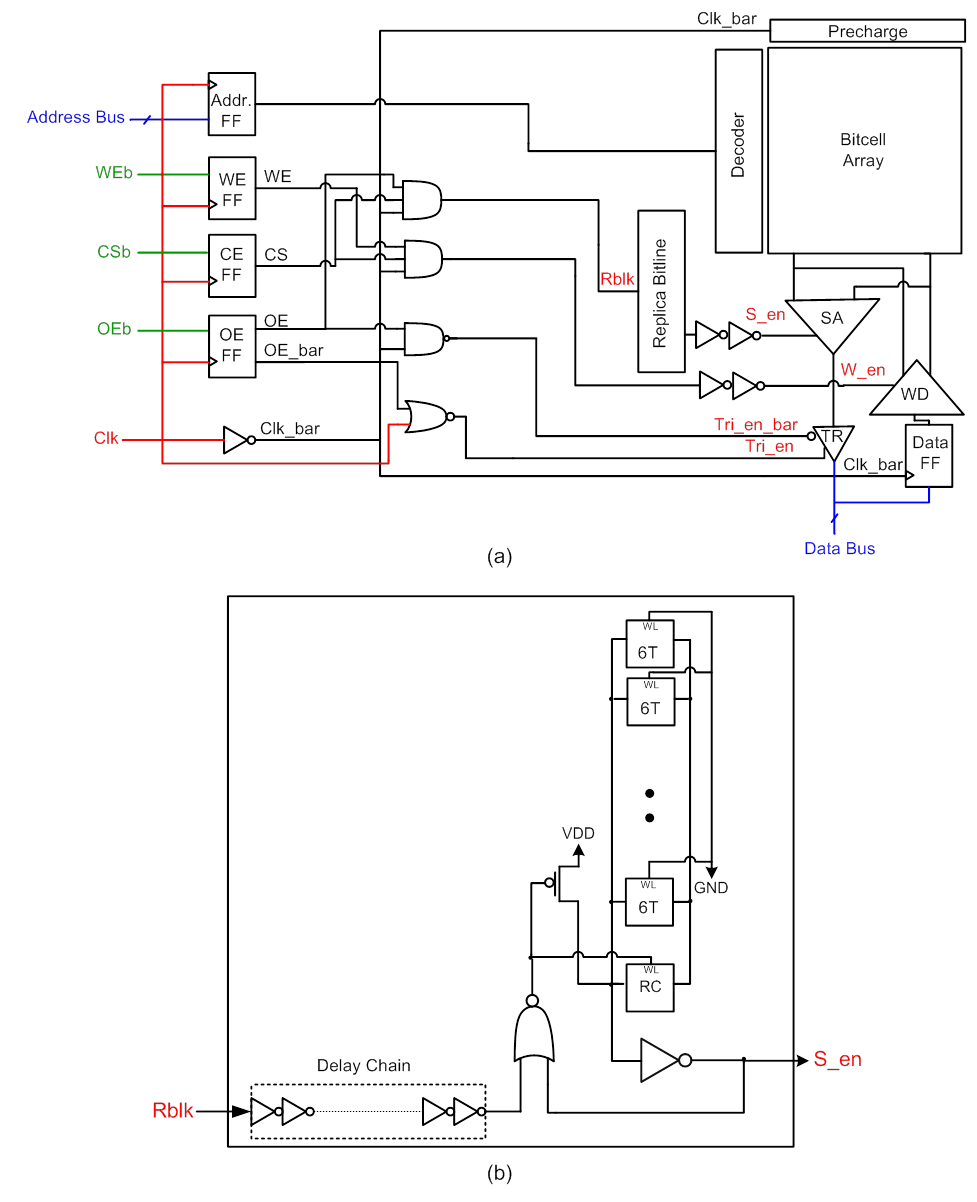
\includegraphics[scale=1]{./figs/control_logic.pdf}
\caption{(a) Control Logic diagram and (b) Replica Bitline Schematic.}
\label{fig:control}
\end{figure}



\begin{table}[h!] 
  \begin{center}
    \begin{tabular}{| c | c | c | c | c | c | c |}
    \hline
    Operation & \multicolumn{3}{|c|}{Inputs} & \multicolumn{3}{|c|}{Outputs}\\ \hline
     & CSb & OEb & WEb & s\_en & w\_en & tri\_en\\ \hline
    READ & 0 & 0 & 1 & 1 & 0 & 1\\ \hline
    WRITE & 0 & 1 & 0 & 0 & 1 & 0\\ \hline
    \end{tabular}
  \end{center}
  \caption{Generation of control signals.}
  \label{table:control}
\end{table}
	 
	 
\subsection{Replica Bitline Delay}
\label{sec:RBL}


	 
In SRAM read operation, discharging the bitline is the most time consuming procedure. 
Generally, sense amplifier amplifies the small voltage difference on the bitlines at the proper sense timing, 
to realize high-speed operation. Therefore, the timing for sense amplifier ($s\_en$) is extremely important for the high speed and low power SRAM. 
If the $s\_en$ arrives early before the bitline difference reaches the sense amplifier input transistors offset voltage, 
a read functional failure may occur. Contrarily, a late-arrived $s\_en$ would consume more unnecessary time, thereby wasting the power. 
The conventional way of generating $s\_en$ signal is to use a replica bitline ($RBL$). $RBL$ as shown in ~\ref{fig:RBL} consists of a column of SRAM cells (dummy cells), 
which track the random process variation in array. $RBL$ is presented for matching the delay of the activation of the 
sense amplifier with the delay of the propagation of the required voltage swing at the bitlines. 
In $RBL$ technique, delay driven memory cell in control path is same as read path. Therefore the 
delay shift of control path according to the Process, Voltage and Temperature (PVT) variation is same ratio as that of read path. 
The $RBL$ technique attains self-timed tracking with optimal $s\_en$ timing according to PVT variation. 
Using replica circuits, the variation on the delay of the sense amp activation and bitline swing is minimized.

\begin{figure}[h!]
\centering
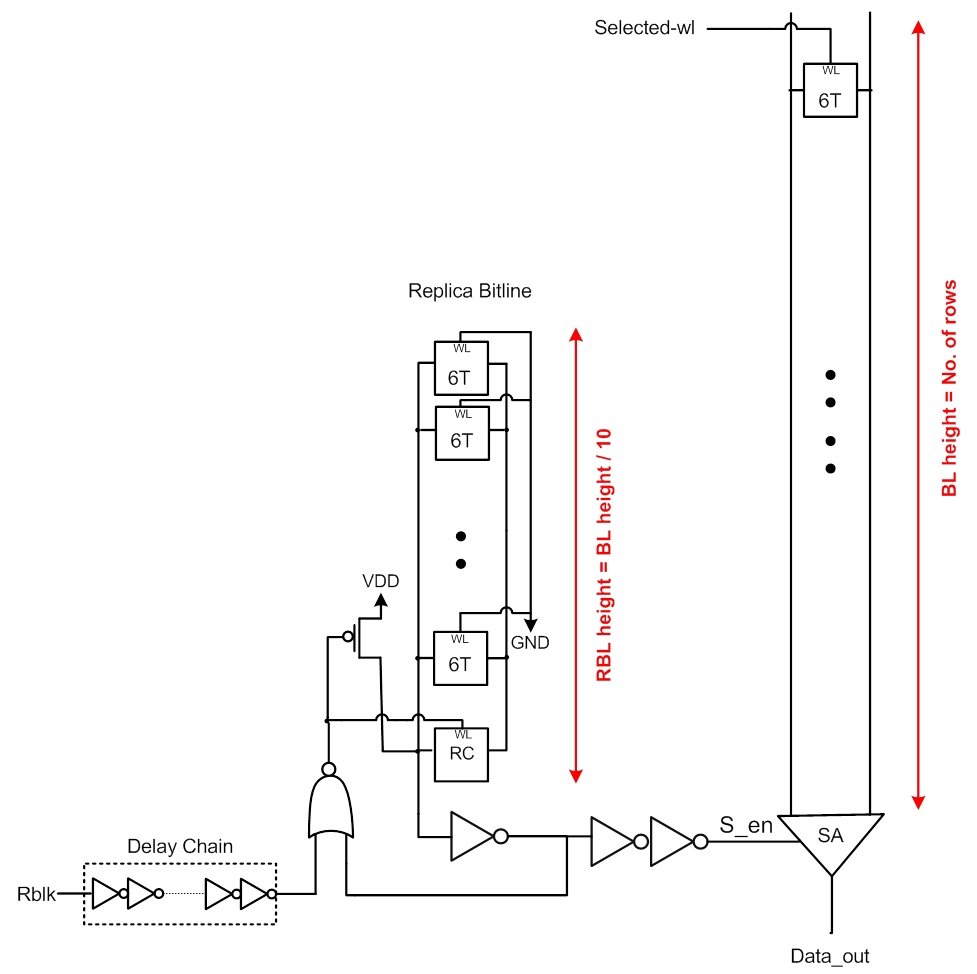
\includegraphics[scale=.9]{./figs/replica_bitline.pdf}
\caption{Replica Bitline Schematic}
\label{fig:RBL}
\end{figure}
 
$RBL$ technique uses a Replica Cell ($RC$) driving a short bitline signal. The short bitline\'s capacitance is set to be a 
fraction of the main bitline capacitance (e.g. one tenth). This fraction is determined by the required bitline swing 
(bitline voltages larger than offset voltage at input transistors of sense amplifier) for proper sensing. So in SRAM, an 
extra column block is converted into the replica column whose capacitance is the desired fraction of the main bitline. 
Therefore, its capacitance ratio to the main bitlines is set purely by the ratio of the geometric lengths (e.g. one tenth). 
The $RC$ is hard wired to store a zero such that it will discharge the $RBL$ once it is accessed. 
Because of its similarity with the actual memory cell (in terms of design and fabrication) the delay of $RBL$ tracks the delay of 
real bitlines very well and can be made roughly equal.  Figure ~\ref{fig:RC} shows the schematic of the 6T replica cell. 
The timing for $s\_en$ is generated as follows. At first, the $RBL$ and the normal bitlines are precharged to VDD. 
Next, selected memory cells and $RC$ are activated.  $RC$ draws the current from the $RBL$ and normal bitlines are 
also discharged through the accessed cell. Discharged swing on $RBL$ is inverted and then buffered to generate the signal to enable the sense amplifier.

	  
\begin{figure}[h!]
\centering
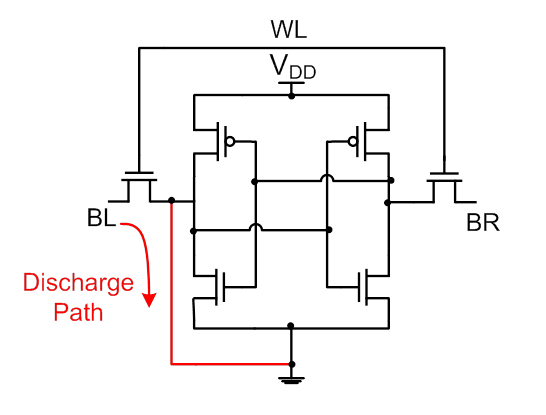
\includegraphics[scale=1]{./figs/replica_cell.pdf}
\caption{Replica Bitline Schematic}
\label{fig:RC}
\end{figure}




\subsection{Timing and Power Characterizer}
\label{characterizer}

The section will provide an explanantion of the characterizer that will generete spice stimuli for the top-level SRAM and perform spice timing simulations to determine the memory setup\&hold times, the write delay, and read delay.  It will also provide a spice power estimate.  



%%%%%%%%%%%%%%%%%%%%%%%%%%%%%%%%%%%%%%%%%%%%%%%%%%%%%%%%%%%%%%%%%%%%%%%%%%%
\section{Unit Tests}
\label{sec:unittests}

OpenRAM comes with a unit testing framework based on the Python
unittest framework. Since OpenRAM is technology independent, these
unit tests can be run in any technology to verify that the technology
is properly ported. By default, FreePDK45 is supported.

The unit tests consist of the following tests that test each module/sub-block of OpenRAM:
\begin{itemize}
\item \verb|00_code_format_check__test.py| - Checks the format of the codes. returns error if finds $TAB$ in codes. 
\item \verb|01_library_drc_test.py| - DRC of library cells in technology \verb|gds_lib|
\item \verb|02_library_lvs_test.py| - LVS of library cells in technology \verb|gds_lib| and \verb|sp_lib| %(names must correspond with different extensions)
\item \verb|03_contact_test.py| - Test contacts/vias of different layers
\item \verb|03_path_test.py| - Test different types of paths based off of the wire module
\item \verb|03_ptx_test.py| - Test various sizes/fingers of PMOS and NMOS parameterized transistors
\item \verb|03_wire_test.py| - Test different types of wires with different layers
\item \verb|04_pinv_test.py|	- Test various sizes of parameterized inverter
\item \verb|04_nand_2_test.py|	- Test various sizes of parameterized nand2
\item \verb|04_nand_3_test.py|	- Test various sizes of parameterized nand3
\item \verb|04_nor_2_test.py|	- Test various sizes of parameterized nor2
\item \verb|04_wordline_driver_test.py|	- Test a wordline\_driver array.
\item \verb|05_array_test.py| - Test a small bit-cell array
\item \verb|06_nand_decoder_test.py|	- Test a dynamic NAND address decoder
\item \verb|06_hierarchical_decoder_test.py|	- Test a dynamic hierarchical address decoder
\item \verb|07_tree_column_mux_test.py| - Test a small tree column mux.
\item \verb|07_single_level_column_mux_test.py| - Test a small single level column mux.
\item \verb|08_precharge_test.py| - Test a dynamically generated precharge array
\item \verb|09_sense_amp_test.py| - Test a sense amplifier array
\item \verb|10_write_driver_test.py| - Test a write driver array
\item \verb|11_ms_flop_array_test.py| - Test a MS\_FF array 
\item \verb|13_control_logic_test.py| - Test the control logic module
\item \verb|14_delay_chain_test.py| - Test a delay chain array
\item \verb|15_tri_gate_array_test.py| - Test a tri-gate array
\item \verb|16_replica_bitline_test.py| - Test a replica bitline
\item \verb|19_bank_test.py| - Test a bank
\item \verb|20_sram_test.py| - Test a complete small SRAM
\item \verb|21_timing_sram_test.py| - Test timing of  SRAM
\item \verb|22_sram_func_test.py| - Test functionality of SRAM
\end {itemize}

Each unit test instantiates a small component and performs DRC/LVS. Automatic DRC/LVS inside OpenRAM is disabled so that Python unittest assertions can be used to track failures, errors, and successful tests as follows:
\begin{verbatim}
        self.assertFalse(calibre.run_drc(a.cell_name,tempgds))
        self.assertFalse(calibre.run_lvs(a.cell_name,tempgds,tempspice))
\end{verbatim}
Each of these assertions will trigger a test failure. If there are
problems with interpreting modified code due to syntax errors, the
unit test framework will not capture this and it will result in an
Error. 

\subsection{Usage}

A regression script is provided to check all of the unit tests by running:
\begin{verbatim}
python tests/regress.py
\end{verbatim}
from the compiler directory located at: "OpenRAM/trunk/compiler/". Each individual test can be run by running:
\begin{verbatim}
python tests/{unit-test file}
e.g. python tests/05_array_test.py
\end{verbatim}
from the compiler directory located at: "openram/trunk/compiler/". As an example, the unit tests all
complete and provide the following output except for the final
\verb|20_sram_test| which has 2 DRC violations:
\begin{verbatim}
[trunk/compiler]$ python tests/regress.py
runTest (01_library_drc_test.library_drc_test) ... ok
runTest (02_library_lvs_test.library_lvs_test) ... ok
runTest (03_contact_test.contact_test) ... ok
runTest (03_path_test.path_test) ... ok
runTest (03_ptx_test.ptx_test) ... ok
runTest (03_wire_test.wire_test) ... ok
runTest (04_pinv_test.pinv_test) ... ok
runTest (04_nand_2_test.nand_2_test) ... ok
runTest (04_nand_3_test.nand_3_test) ... ok
runTest (04_nor_2_test.nor_2_test) ... ok
runTest (04_wordline_driver_test.wordline_driver_test) ... ok
runTest (05_array_test.array_test) ... ok
runTest (06_hierdecoder_test.hierdecoder_test) ... ok
runTest (07_single_level_column_mux_test.single_level_column_mux_test) ... ok
runTest (08_precharge_test.precharge_test) ... ok
runTest (09_sense_amp_test.sense_amp_test) ... ok
runTest (10_write_driver_test.write_driver_test) ... ok
runTest (11_ms_flop_array_test.ms_flop_test) ... ok
runTest (13_control_logic_test.control_logic_test) ... ok
runTest (14_delay_chain_test.delay_chain_test) ... ok
runTest (15_tri_gate_array_test.tri_gate_array_test) ... ok
runTest (19_bank_test.bank_test) ... ok
runTest (20_sram_test.sram_test) ... ok  
\end{verbatim}

If there are any DRC/LVS violations during the test, all the summary,output,and error files
will be generated in the technology directory's "openram\_temp" folder. One would view those
files to determine the cause of the DRC/LVS violations.

More information on the Python unittest framework is available at\\
\begin{center}
\url{http://docs.python.org/2/library/unittest.html}.
\end{center}


%%%%%%%%%%%%%%%%%%%%%%%%%%%%%%%%%%%%%%%%%%%%%%%%%%%%%%%%%%%%%%%%%%%%%%%%%%%
\section{Debug Framework}
\label{sec:debug}

All output in OpenRAM should use the shared debug framework. This is
still under development but is in a usable state. It is going to be
replaced with the Python Logging framework which is quite simple.

All of the debug framework is contained in debug.py and is based
around the concept of a ``debug level'' which is a single global
variable in this file. This level is, by default, 0 which will output
normal minimal output. The general guidelines for debug output are:
\begin{itemize}
\item 0 Normal output
\item 1 Verbose output
\item 2 Detailed output
\item 3+ Excessively detailed output
\end{itemize}

The debug level can be adjusted on the command line when arguments are parsed using the ``-v'' flag. Adding more ``-v'' flags will increase the debug level as in the following examples:
\begin{verbatim}
python tests/01_library_drc_test.py -vv
python openram.py 4 16 -v -v
\end{verbatim}
which each put the program in debug level 2 (detailed output).

Since every module may output a lot of information in the higher debug
levels, the output format is standardized to allow easy searching via
grep or other command-line tools. The standard output formatting is
used through three interface functions: 
\begin{itemize}
\item debug.info(int, msg)
\item debug.warning(msg)
\item debug.error(msg)
\end{itemize}
The msg string in each case can be any string format including data or
other useful debug information. The string should also contain
information to make it human understandable. {\bf It should not just be
  a number!} The warning and error messages are independent of debug
levels while the info message will only print the message if the
current debug level is above the parameter value.

The output format of the debug info messages are:
\begin{verbatim}
[ module ]:  msg
\end{verbatim}
where module is the calling module name and msg is the string
provided. This enables a grep command to get the relevant lines.  The
warning and error messages include the file name and line number of
the warning/error.


%%%%%%%%%%%%%%%%%%%%%%%%%%%%%%%%%%%%%%%%%%%%%%%%%%%%%%%%%%%%%%%%%%%%%%%%%%%
%\input{conclusions}
\section*{GDSMill}
\label{sec:gdsMill_permission}

OpenRAM uses gdsMill, a GDS library written by Michael Wieckowski at
the University of Michigan. Michael gave us complete permission to use
the code. Since then, we have made several bug and performance
enhancements to gdsMill. In addition, gdsMill is no longer available
on the web, so we distribute it along with OpenRAM.


\begin{verbatim}
From: Michael Wieckowski <wieckows@umich.edu>
Date: Thu, Oct 14, 2010 at 12:49 PM
Subject: Re: GDS Mill
To: Matthew Guthaus <mrg@soe.ucsc.edu>

Hi Matt,

Feel free to use / modify / distribute the code as you like.

-Mike

On Oct 14, 2010, at 3:07 PM, Matthew Guthaus wrote:
> Hi Michael (& Dennis),
>
> A student and I were looking at your GDS tools, but 
> we noticed that there is no license. What is the license?
>
> Thanks,
>
> Matt

\end{verbatim}



\end{document}
